% =====================================================================================
% Grover's Search Algorithm - explained for first-year engineering students
% Build:  python make_figures.py   (needs cudaq, numpy, matplotlib; run it on Linux, for example in WSL)
%         latexmk -pdf grover_lecture.tex
% =====================================================================================
\documentclass[aspectratio=169,11pt]{beamer}
\usepackage[T1]{fontenc}
\usepackage{lmodern}
\usepackage{amsmath,amssymb}
\usepackage{braket}
\usepackage{graphicx}
\usepackage{booktabs}
\usepackage{array}
\usepackage{tikz}
\usepackage{quantikz}
\usepackage{listings}
\graphicspath{{figures/}}
\newcommand{\nthreerows}{%
  start $\ket{s}$ & $+0.3536$ & $+0.3536$ & $0.1250$\\
  after $U_\omega$ & $+0.3536$ & $-0.3536$ & $0.1250$\\
  after $D$ ($k = 1$) & $+0.1768$ & $+0.8839$ & $0.7812$\\
  after $U_\omega$ again & $+0.1768$ & $-0.8839$ & $0.7812$\\
  after $D$ ($k = 2$) & $-0.0884$ & $+0.9723$ & $0.9453$\\
}

\newcommand{\devsix}{6.2e-14}
\newcommand{\marksfifteen}{1999}
\newcommand{\timefifteen}{38.6}
\newcommand{\hcount}{4275}
\newcommand{\xcount}{5964}
\newcommand{\benchrows}{%
  6 & 6 & 0.05 & 1990\\
  7 & 8 & 0.44 & 1993\\
  8 & 12 & 0.02 & 2000\\
  9 & 17 & 0.04 & 1997\\
  10 & 25 & 0.18 & 1999\\
  11 & 35 & 0.23 & 2000\\
  12 & 50 & 0.85 & 2000\\
  13 & 71 & 2.69 & 2000\\
  14 & 100 & 9.02 & 2000\\
  15 & 142 & 38.58 & 1999\\
}
\newcommand{\shotsrows}{%
  0 & 0.0625 & 123 & 0.0615\\
  1 & 0.4727 & 942 & 0.4710\\
  3 & 0.9613 & 1922 & 0.9610\\
}
\newcommand{\noisefour}{0.882}
\newcommand{\noiseone}{0.628}
\newcommand{\noisethree}{0.305}
\newcommand{\hostinfo}{Linux, 12 logical CPUs, CUDA-Q 0.16.0}


% ---- colours and look (identical to the QFT lecture) -----------------------------------
\definecolor{qblue}{HTML}{2A78D6}
\definecolor{qdark}{HTML}{1C5CAB}
\definecolor{qorange}{HTML}{EB6834}
\definecolor{qaqua}{HTML}{1BAF7A}
\definecolor{qink}{HTML}{0B0B0B}
\definecolor{qgrey}{HTML}{52514E}
\definecolor{qlight}{HTML}{EEF4FC}
\setbeamercolor{structure}{fg=qdark}
\setbeamercolor{frametitle}{fg=qdark}
\setbeamercolor{title}{fg=qdark}
\setbeamercolor{normal text}{fg=qink}
\setbeamercolor{block title}{bg=qblue,fg=white}
\setbeamercolor{block body}{bg=qlight,fg=qink}
\setbeamercolor{block title example}{bg=qaqua,fg=white}
\setbeamercolor{block body example}{bg=qaqua!10,fg=qink}
\setbeamercolor{block title alerted}{bg=qorange,fg=white}
\setbeamercolor{block body alerted}{bg=qorange!10,fg=qink}
\setbeamertemplate{blocks}[rounded][shadow=false]
\setbeamertemplate{navigation symbols}{}
\setbeamertemplate{itemize items}[circle]
\setbeamertemplate{enumerate items}[default]
\setbeamerfont{frametitle}{size=\large,series=\bfseries}
% =====================================================================================
% SILICO FELLER branding for the beamer lecture decks (16:9).
% \input this file in the preamble of every presentations/<algorithm>_source/<algorithm>_lecture.tex,
% after graphicx is loaded and the colours/fonts are set. It is the "slide master":
%   * the official logo (assets/branding/silico_feller_logo.png, unmodified, aspect ratio kept)
%     is drawn at the top-right of EVERY slide through the background template, so new or
%     re-ordered slides get it automatically;
%   * the frame-title box is narrowed on the right so titles wrap before they can reach the logo.
% =====================================================================================
\makeatletter
\newcommand{\sflogofile}{../../assets/branding/silico_feller_logo.png}
\newlength{\sflogoheight}\setlength{\sflogoheight}{5.4mm}   % logo height on the slide (width follows the aspect ratio)
\newlength{\sflogomargin}\setlength{\sflogomargin}{2.5mm}   % distance from the top and right paper edges
\newlength{\sflogoreserve}\setlength{\sflogoreserve}{2.6cm} % horizontal space kept free for the logo in the title row

% logo on every slide (background layer: never covers slide content)
\setbeamertemplate{background}{%
  \vbox to \paperheight{%
    \vskip\sflogomargin
    \hbox to \paperwidth{\hfill\includegraphics[height=\sflogoheight]{\sflogofile}\hskip\sflogomargin}%
    \vfill}}

% frame title: same look as beamer's default, but it stops \sflogoreserve before the right edge
\setbeamertemplate{frametitle}{%
  \ifbeamercolorempty[bg]{frametitle}{}{\nointerlineskip}%
  \begin{beamercolorbox}[sep=0.3cm,left,wd=\paperwidth]{frametitle}%
    \usebeamerfont{frametitle}%
    \vbox{}\vskip-1ex%
    \parbox[t]{\dimexpr\paperwidth-0.6cm-\sflogoreserve\relax}{\raggedright
      \strut\insertframetitle\strut\par
      \ifx\insertframesubtitle\@empty\else
        {\usebeamerfont{framesubtitle}\usebeamercolor[fg]{framesubtitle}\insertframesubtitle\strut\par}%
      \fi}%
    \vskip-1ex%
    \vskip-.3cm%
  \end{beamercolorbox}}
\makeatother
   % SILICO FELLER logo on every slide
\setbeamertemplate{footline}{%
  \leavevmode\hbox{\begin{beamercolorbox}[wd=\paperwidth,ht=2.4ex,dp=1ex,leftskip=0.4cm,rightskip=0.4cm]{normal text}%
    \color{qgrey}\tiny Grover's Search Algorithm\ \ $\cdot$\ \ \insertsectionhead\hfill\insertframenumber\,/\,\inserttotalframenumber
  \end{beamercolorbox}}}
\newcommand{\hl}[1]{{\color{qorange}\textbf{#1}}}
\newcommand{\key}[1]{{\color{qdark}\textbf{#1}}}
\newcommand{\kopt}{k_{\rm opt}}
\newcommand{\xs}{x^\ast}
\newcommand{\Uo}{U_\omega}
\newcommand{\pj}[1]{\ket{#1}\!\bra{#1}}

\lstset{language=Python, basicstyle=\ttfamily\scriptsize, keywordstyle=\color{qdark}\bfseries,
  commentstyle=\color{qgrey}\itshape, stringstyle=\color{qorange}, showstringspaces=false,
  frame=single, rulecolor=\color{qblue!40}, backgroundcolor=\color{qlight}, columns=fullflexible}

\title{Grover's Search Algorithm}
\subtitle{From looking through a list to quantum amplitude amplification --- explained step by step}
\author{CUDA-Q Quantum Algorithm Benchmarking Suite}
\date{For first-year engineering students}

\begin{document}

% =====================================================================================
\section{Introduction}
\begin{frame}
  \titlepage
  \centering\small\color{qgrey}
  Quantum results come from NVIDIA CUDA-Q on its CPU simulators, checked against theory. No GPU or quantum hardware run is shown.
\end{frame}

\begin{frame}{What you will learn today}
  \begin{columns}[T]
    \begin{column}{0.55\textwidth}
      \small
      \begin{enumerate}
        \item What a \key{search problem} is and what it costs classically
        \item The math toolkit: \key{complex numbers}, vectors, reflections
        \item \key{Qubits} in ten minutes
        \item \key{Grover's algorithm}: oracle, diffusion, iteration
        \item The \key{geometric picture} and every derivation
        \item Several solutions, unknown $M$, amplification, counting
        \item How to \key{build the circuit} from simple gates
        \item The \key{CUDA-Q notebook}, measured results, noise and limits
      \end{enumerate}
    \end{column}
    \begin{column}{0.42\textwidth}
      \begin{block}{You only need}
        \begin{itemize}
          \item school algebra (powers, sums)
          \item vectors and matrices (multiplying a matrix by a vector)
          \item a little trigonometry ($\sin$, $\cos$)
        \end{itemize}
        Everything else is explained on the way.
      \end{block}
    \end{column}
  \end{columns}
\end{frame}

\begin{frame}{Symbols used in every slide}
  \begin{columns}[T]
    \begin{column}{0.5\textwidth}
      \small
      \begin{tabular}{ll}
        \toprule
        symbol & meaning\\
        \midrule
        $n$ & number of qubits\\
        $N = 2^n$ & number of items searched\\
        $M$ & number of marked items\\
        $x$ & an item, as an $n$-bit string\\
        $\xs$ & the marked item (when $M = 1$)\\
        $f(x)$ & 1 if $x$ is marked, otherwise 0\\
        $\Uo$ & phase oracle\\
        $D$ & diffusion operator\\
        $G = D\Uo$ & one Grover iteration\\
        $k$ & number of iterations\\
        $\theta$ & angle with $\sin\theta = \sqrt{M/N}$\\
        \bottomrule
      \end{tabular}
    \end{column}
    \begin{column}{0.46\textwidth}
      \begin{block}{Reading convention}
        Qubit 1 (top wire) is the \hl{most significant bit}: $\ket{101}$ is the number 5.
      \end{block}
      \vspace{1mm}
      \begin{alertblock}{Notebook naming}
        \texttt{Grover.ipynb} uses $N$ for the number of qubits, $M = 2^N$ for the items, and $O$ for the oracle. The formulas are the same; only the letters differ.
      \end{alertblock}
    \end{column}
  \end{columns}
\end{frame}

% =====================================================================================
\section{Part 1: Why search is hard}
\begin{frame}{What is a search problem?}
  \begin{columns}[T]
    \begin{column}{0.52\textwidth}
      \begin{itemize}
        \item We have $N$ possible candidates (the \key{search space}).
        \item We can \key{check} a candidate quickly.
        \item We want a candidate that passes the check.
      \end{itemize}
      \vspace{2mm}
      \begin{block}{Examples}
        \begin{itemize}
          \item Which password opens this file?
          \item Which assignment of $n$ true/false variables satisfies these rules?
          \item Which route is shorter than 500 km?
        \end{itemize}
      \end{block}
    \end{column}
    \begin{column}{0.44\textwidth}
      \begin{exampleblock}{The common idea}
        \centering \textbf{Checking is easy, finding is hard.}\\[1mm]
        \raggedright A checker is short code, but the list of candidates can be astronomically long.
      \end{exampleblock}
      \vspace{1mm}
      $n$ bits give $N = 2^n$ candidates:\\
      $n = 20$: about a million.\\
      $n = 40$: about a trillion.
    \end{column}
  \end{columns}
\end{frame}

\begin{frame}{Classical search: structure decides the cost}
  \begin{columns}[T]
    \begin{column}{0.48\textwidth}
      \begin{block}{Sorted list: binary search}
        Compare with the middle, discard half, repeat.\\[1mm]
        Worst case: about $\log_2 N$ comparisons.\\
        $N = 1023$: at most $10$.
      \end{block}
    \end{column}
    \begin{column}{0.48\textwidth}
      \begin{alertblock}{Unsorted list: linear search}
        No order to use: look at the items one by one.\\[1mm]
        Worst case: $N$ comparisons.\\
        $N = 1023$: up to $1023$.
      \end{alertblock}
    \end{column}
  \end{columns}
  \vspace{3mm}
  \begin{itemize}
    \item Grover's algorithm is about the second case: \key{unstructured search}.
    \item If your data is sorted, classical binary search is much faster than Grover. Quantum does not beat everything.
  \end{itemize}
\end{frame}

\begin{frame}{The black-box model: we count queries}
  \begin{columns}[T]
    \begin{column}{0.54\textwidth}
      The only access to the problem is a function
      \[ f(x) = \begin{cases} 1 & x \text{ is marked}\\ 0 & \text{otherwise}\end{cases} \]
      \begin{itemize}
        \item $f$ is the \key{oracle}: a black box that recognises a solution.
        \item One use of $f$ is one \key{query}.
        \item Cost = number of queries.
      \end{itemize}
    \end{column}
    \begin{column}{0.42\textwidth}
      \begin{alertblock}{Query cost is not total cost}
        Each query also costs gates. In practice:
        \[ \text{total work} = \text{queries} \times \text{cost per query}. \]
        Keep these two apart when you read any speed-up claim.
      \end{alertblock}
    \end{column}
  \end{columns}
\end{frame}

\begin{frame}{How expensive is classical search?}
  \begin{columns}[T]
    \begin{column}{0.5\textwidth}
      Picking cards one at a time, without putting them back, $M$ marked among $N$:
      \begin{block}{Expected number of queries}
        \[ \frac{N + 1}{M + 1} \]
      \end{block}
      \small
      Why: the $M$ marked cards cut the others into $M + 1$ gaps of equal average size.\\[1mm]
      \normalsize
      Big-O notation: the classical cost is $\Theta(N/M)$.
    \end{column}
    \begin{column}{0.46\textwidth}
      \begin{exampleblock}{Worked example}
        $N = 31$, $M = 3$: $\frac{32}{4} = 8$ draws.\\[1mm]
        Check: $28$ unmarked in $4$ gaps gives $7$ before the first marked card; it is draw number $8$.
      \end{exampleblock}
      \vspace{1mm}
      One marked item: $\frac{N+1}{2} \approx \frac N2$ on average, $N$ in the worst case. $N = 2^{15}$: about $16\,384$.
    \end{column}
  \end{columns}
\end{frame}

\begin{frame}{The quantum idea (preview)}
  \begin{columns}[c]
    \begin{column}{0.48\textwidth}
      \begin{block}{Grover's result}
        Find a marked item with about
        \[ \frac\pi4\sqrt{\frac NM}\ \text{ queries.} \]
      \end{block}
      \small
      \begin{tabular}{rrr}
        \toprule
        $N$ & classical $\frac N2$ & Grover\\
        \midrule
        $2^{15}$ & $16\,384$ & $142$\\
        $2^{20}$ & $524\,288$ & $804$\\
        $2^{30}$ & $5.4\times10^{8}$ & $25\,735$\\
        \bottomrule
      \end{tabular}
    \end{column}
    \begin{column}{0.48\textwidth}
      \centering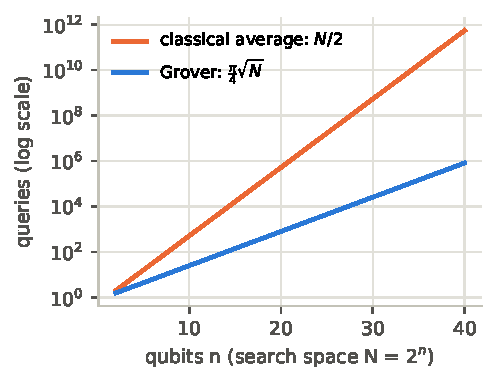
\includegraphics[width=\textwidth]{search_cost}\\
      \small A \hl{quadratic} speed-up: large, but not exponential.
    \end{column}
  \end{columns}
\end{frame}

\begin{frame}{``Quantum parallelism'': what it does and does not mean}
  \begin{columns}[T]
    \begin{column}{0.48\textwidth}
      \key{True}: one oracle call on a superposition acts on all $N$ basis states:
      \[ \Uo\sum_x c_x\ket{x} = \sum_x (-1)^{f(x)}c_x\ket{x}. \]
      \vspace{1mm}
      \key{False}: ``it tries all answers and gives you the right one''. A measurement returns \hl{one} random $x$.
    \end{column}
    \begin{column}{0.48\textwidth}
      \begin{alertblock}{The real challenge}
        After one oracle call each outcome is still equally likely.\\[1mm]
        We must make the amplitude of the marked item \hl{grow} through interference, a little at each step.
      \end{alertblock}
      \vspace{1mm}
      That is why Grover needs $\sim\sqrt N$ queries and not just one.
    \end{column}
  \end{columns}
\end{frame}

% =====================================================================================
\section{Part 2: Math toolkit}
\begin{frame}{Complex numbers and phases}
  \begin{columns}[T]
    \begin{column}{0.52\textwidth}
      A complex number $z = a + ib$ with $i^2 = -1$:
      \begin{itemize}
        \item \key{modulus} $|z| = \sqrt{a^2 + b^2}$ (length)
        \item \key{polar form} $z = |z|e^{i\varphi}$, with $\varphi$ the angle
        \item \key{conjugate} $\bar z = a - ib$, and $|z|^2 = \bar zz$
      \end{itemize}
      \begin{block}{Euler's formula}
        \[ e^{i\varphi} = \cos\varphi + i\sin\varphi, \qquad |e^{i\varphi}| = 1 \]
      \end{block}
    \end{column}
    \begin{column}{0.44\textwidth}
      \begin{exampleblock}{Worked example}
        $z = \frac{1 + i}{\sqrt2} = e^{i\pi/4}$ has modulus 1.\\[1mm]
        $z^6 = e^{6i\pi/4} = e^{3i\pi/2} = -i$.
      \end{exampleblock}
      \vspace{1mm}
      \key{The value $-1$ is a phase}: $-1 = e^{i\pi}$. Grover's oracle multiplies amplitudes by exactly this number. It changes the direction, never the length.
    \end{column}
  \end{columns}
\end{frame}

\begin{frame}{Vectors, inner products and normalisation}
  \begin{columns}[T]
    \begin{column}{0.53\textwidth}
      Quantum states are vectors of complex numbers: a \key{Hilbert space} is the vector space $\mathbb{C}^N$ together with this inner product:
      \begin{block}{Inner product}
        \[ \braket{u|v} = \sum_k\overline{u_k}\,v_k \]
      \end{block}
      \begin{itemize}
        \item Length: $\|v\|^2 = \braket{v|v} = \sum_k|v_k|^2$
        \item Normalised: length 1. Orthogonal: $\braket{u|v} = 0$
        \item Note the bar: conjugate the \hl{first} vector.
      \end{itemize}
    \end{column}
    \begin{column}{0.43\textwidth}
      \begin{exampleblock}{Worked example}
        Normalise $(1, i, 1 + i, 2)$:\\[1mm]
        $|1|^2 + |i|^2 + |1 + i|^2 + |2|^2$\\
        $= 1 + 1 + 2 + 4 = 8$,\\[1mm]
        so multiply by $c = \frac{1}{2\sqrt2}$.
      \end{exampleblock}
      \vspace{1mm}
      \small \key{Computational basis}: the unit vectors $e_0, \dots, e_{N-1}$. For qubits they are written $\ket{0}, \dots, \ket{N-1}$. Each is one item of the search space.
    \end{column}
  \end{columns}
\end{frame}

\begin{frame}{The trigonometry we need}
  \begin{columns}[c]
    \begin{column}{0.48\textwidth}
      \begin{block}{Identities}
        \[ \cos2\alpha = 1 - 2\sin^2\alpha \]
        \[ \sin2\alpha = 2\sin\alpha\cos\alpha \]
        \[ \sin3\alpha = 3\sin\alpha - 4\sin^3\alpha \]
      \end{block}
      \begin{exampleblock}{Worked example}
        $\sin\theta = \frac14$: $\ \sin3\theta = \frac34 - \frac{4}{64} = \frac{11}{16}$, so $\sin^2 3\theta = \frac{121}{256}$.
      \end{exampleblock}
    \end{column}
    \begin{column}{0.48\textwidth}
      \centering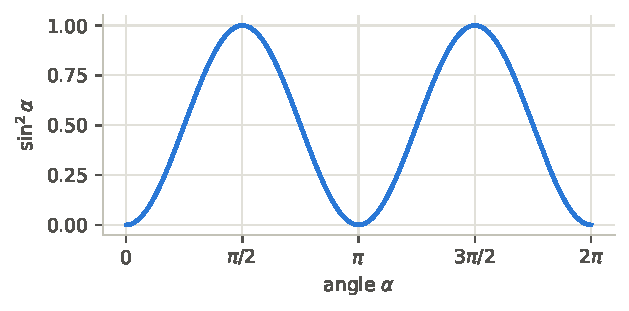
\includegraphics[width=\textwidth]{sin2_curve}\\
      \raggedright\small
      $\sin^2\alpha$ repeats every $\pi$ (not $2\pi$) and equals 1 at odd multiples of $\frac\pi2$. Remember the shape: the success probability of Grover follows it.
    \end{column}
  \end{columns}
\end{frame}

\begin{frame}{Reflections are simple matrices}
  \begin{columns}[T]
    \begin{column}{0.52\textwidth}
      For a unit vector $\ket{u}$:
      \begin{block}{Reflection about $\ket{u}$}
        \[ R_u = 2\pj{u} - I \]
      \end{block}
      \begin{itemize}
        \item $\pj{u}$ is the matrix with entries $u_j\overline{u_k}$ (the \key{projector} on $\ket{u}$).
        \item $R_u\ket{u} = \ket{u}$: the axis stays.
        \item $R_u\ket{w} = -\ket{w}$ if $\braket{u|w} = 0$.
        \item $R_u^2 = I$: reflecting twice undoes it.
      \end{itemize}
    \end{column}
    \begin{column}{0.44\textwidth}
      \begin{exampleblock}{Worked example}
        $u = (\frac35, \frac45)$:
        \[ 2uu^{T} - I = \frac{1}{25}\begin{pmatrix}-7 & 24\\ 24 & 7\end{pmatrix} \]
        Check: it maps $u$ to $u$; trace $0$, determinant $-1$.
      \end{exampleblock}
      \small $\pj{u}$ alone is \hl{not} unitary (it has eigenvalue 0); $R_u$ is.
    \end{column}
  \end{columns}
\end{frame}

\begin{frame}{Two reflections make a rotation}
  \centering
  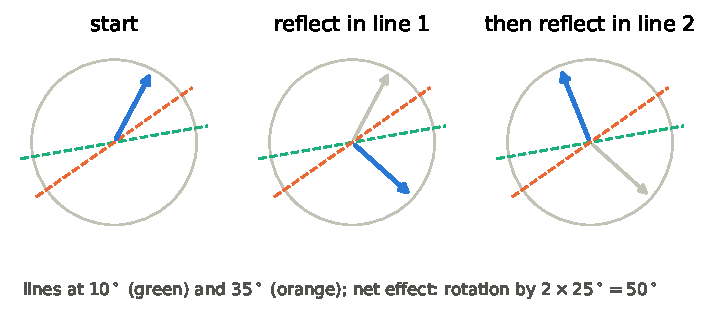
\includegraphics[width=0.74\textwidth]{two_reflections}\\[-1mm]
  \raggedright
  \begin{columns}[T]
    \begin{column}{0.5\textwidth}
      A reflection in the line at angle $\alpha$ sends angle $\phi$ to $2\alpha - \phi$. Reflect at $\alpha$, then at $\beta$:
      \[ \phi \to 2\alpha - \phi \to 2\beta - 2\alpha + \phi. \]
    \end{column}
    \begin{column}{0.46\textwidth}
      \begin{alertblock}{Remember this}
        The result is a rotation by \hl{twice the angle between the lines}. Grover is exactly this.
      \end{alertblock}
    \end{column}
  \end{columns}
\end{frame}

\begin{frame}{Inversion about the mean}
  \centering
  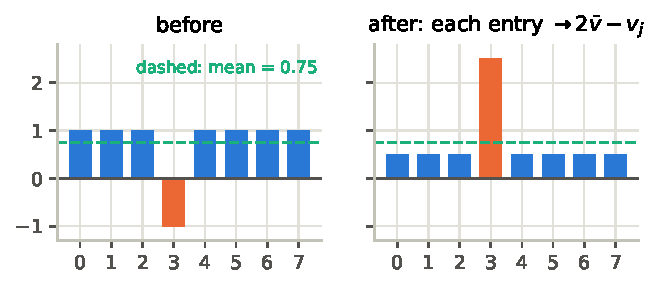
\includegraphics[width=0.66\textwidth]{mean_inversion}\\
  \raggedright
  \begin{columns}[T]
    \begin{column}{0.56\textwidth}
      For a list with mean $\bar v$: $\ v_j \mapsto 2\bar v - v_j$. A value a distance $d$ below the mean ends a distance $d$ above it.
      Example: seven $+1$ and one $-1$: $\bar v = \frac34$; the $-1$ becomes $\frac52$, the others $\frac12$.
    \end{column}
    \begin{column}{0.4\textwidth}
      \begin{block}{Check}
        The sum of squares stays the same: $7\cdot\frac14 + \frac{25}{4} = 8 = 7 + 1$.
      \end{block}
    \end{column}
  \end{columns}
\end{frame}

% =====================================================================================
\section{Part 3: Qubits in ten minutes}
\begin{frame}{Bit vs. qubit}
  \begin{columns}[T]
    \begin{column}{0.46\textwidth}
      A classical \key{bit} is 0 or 1.\\[2mm]
      A \key{qubit} is a unit vector of two complex numbers:
      \[ \ket{0} = \begin{pmatrix}1\\0\end{pmatrix}, \quad \ket{1} = \begin{pmatrix}0\\1\end{pmatrix} \]
      \[ \ket{\psi} = \alpha\ket{0} + \beta\ket{1} = \begin{pmatrix}\alpha\\ \beta\end{pmatrix} \]
      with $|\alpha|^2 + |\beta|^2 = 1$.
      $\alpha, \beta$ are called \key{amplitudes}.
    \end{column}
    \begin{column}{0.44\textwidth}
      \begin{exampleblock}{Superposition}
        \[ \ket{\pm} = \tfrac{1}{\sqrt2}\big(\ket{0} \pm \ket{1}\big) \]
        are vectors with two non-zero components --- ``0 and 1 at the same time'' in that precise sense.
      \end{exampleblock}
      \vspace{2mm}
      The notation $\ket{\cdot}$ (``ket'') just marks a column vector; $\bra{\cdot}$ (``bra'') is its conjugate row vector.
    \end{column}
  \end{columns}
\end{frame}

\begin{frame}{Measurement: amplitudes become probabilities}
  \begin{block}{Born rule}
    Measuring $\sum_x c_x\ket{x}$ gives $x$ with probability $|c_x|^2$. Afterwards the register \emph{is} in the state $\ket{x}$.
  \end{block}
  \centering
  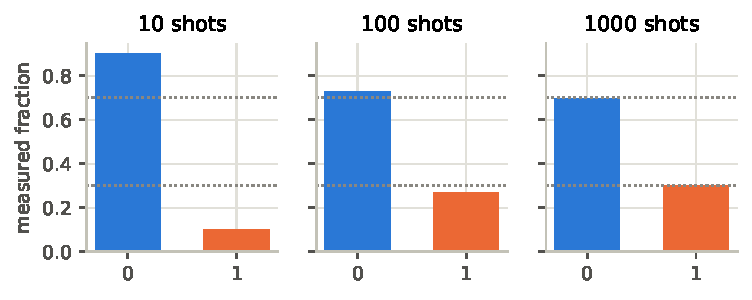
\includegraphics[width=0.8\textwidth]{measurement_shots}\\
  \raggedright\small
  A qubit with $|\alpha|^2 = 0.7$ measured 10, 100 and 1000 times (CUDA-Q). One \key{shot} gives one bit; the
  probabilities only appear after many shots (dotted lines: 0.7 and 0.3).
\end{frame}

\begin{frame}{Many qubits: registers and tensor products}
  \begin{itemize}
    \item $n$ qubits (a \key{register}) have $2^n$ basis states, one for each $n$-bit string:
      \[ \ket{\psi} = \sum_{x=0}^{2^n-1} c_x \ket{x}, \qquad \sum_x |c_x|^2 = 1 . \]
    \item Independent qubits combine with the \key{tensor product}:
      \[ (a_0\ket0 + a_1\ket1)\otimes(b_0\ket0 + b_1\ket1) = a_0b_0\ket{00} + a_0b_1\ket{01} + a_1b_0\ket{10} + a_1b_1\ket{11} \]
    \item Example: $\frac{1}{\sqrt2}(\ket0 + i\ket1)\otimes\frac{1}{\sqrt2}(\ket0 - \ket1)$ has the amplitude $\frac i2$ on $\ket{10}$.
  \end{itemize}
  \begin{alertblock}{Why simulation is hard}
    A classical computer stores all $2^n$ complex numbers, 16 bytes each: $n = 30$ needs 16\,GiB, and $n = 50$ needs 16\,PiB.
  \end{alertblock}
\end{frame}

\begin{frame}{Single-qubit gates are $2\times 2$ matrices}
  \begin{columns}[T]
    \begin{column}{0.32\textwidth}
      \begin{block}{NOT gate $X$}
        \[ X = \begin{pmatrix}0&1\\1&0\end{pmatrix} \]
        $X\ket0 = \ket1$, $X\ket1 = \ket0$
      \end{block}
    \end{column}
    \begin{column}{0.32\textwidth}
      \begin{block}{Phase flip $Z$}
        \[ Z = \begin{pmatrix}1&0\\0&-1\end{pmatrix} \]
        $Z\ket0 = \ket0$, $Z\ket1 = -\ket1$
      \end{block}
    \end{column}
    \begin{column}{0.32\textwidth}
      \begin{block}{Hadamard $H$}
        \[ H = \tfrac{1}{\sqrt2}\begin{pmatrix}1&1\\1&-1\end{pmatrix} \]
        $H\ket0 = \ket+$, $H\ket1 = \ket-$
      \end{block}
    \end{column}
  \end{columns}
  \vspace{3mm}
  \begin{itemize}
    \item Useful facts: $HXH = Z$, $\ HZH = X$, $\ X\ket\pm = \pm\ket\pm$, $\ Z\ket\pm = \ket\mp$.
    \item Gates are \key{unitary}: $U^\dagger U = I$. They keep the vector length 1 and can always be undone.
    \item $U^\dagger$ means ``transpose and conjugate''. Measurements are not unitary; projectors are not gates.
  \end{itemize}
\end{frame}

\begin{frame}{The Pauli gates $X$, $Y$ and $Z$}
  \begin{columns}[T]
    \begin{column}{0.32\textwidth}
      \begin{block}{$X$: bit flip}
        \[ X = \begin{pmatrix}0&1\\1&0\end{pmatrix} \]
        $X\ket0 = \ket1$, $X\ket1 = \ket0$
      \end{block}
    \end{column}
    \begin{column}{0.32\textwidth}
      \begin{block}{$Y$: bit and phase flip}
        \[ Y = \begin{pmatrix}0&-i\\i&0\end{pmatrix} \]
        $Y\ket0 = i\ket1$, $Y\ket1 = -i\ket0$
      \end{block}
    \end{column}
    \begin{column}{0.32\textwidth}
      \begin{block}{$Z$: phase flip}
        \[ Z = \begin{pmatrix}1&0\\0&-1\end{pmatrix} \]
        $Z\ket0 = \ket0$, $Z\ket1 = -\ket1$
      \end{block}
    \end{column}
  \end{columns}
  \vspace{2mm}
  \begin{columns}[T]
    \begin{column}{0.54\textwidth}
      \begin{itemize}
        \item Each \key{Pauli} matrix $P$ is Hermitian and unitary: $P^2 = I$, with eigenvalues $\pm1$.
        \item Products: $XY = iZ$, $\ YZ = iX$, $\ ZX = iY$.
        \item Different Paulis anticommute: $XZ = -ZX$.
      \end{itemize}
    \end{column}
    \begin{column}{0.42\textwidth}
      \begin{exampleblock}{Worked example}
        $Y\ket{+} = \tfrac{1}{\sqrt2}\big(i\ket1 - i\ket0\big) = -i\ket{-}$.
      \end{exampleblock}
      \small \hl{In Grover}: $X$ relabels states and a multi-controlled $Z$ flips a sign. The notebook's circuit does not use $Y$.
    \end{column}
  \end{columns}
\end{frame}

\begin{frame}{Hadamard layer: state preparation for search}
  Apply $H$ to every qubit of $\ket{0\dots0}$ (the \key{state preparation} step):
  \begin{block}{Uniform superposition}
    \[ \ket{s} = H^{\otimes n}\ket{0}^{\otimes n} = \ket{+}^{\otimes n} = \frac{1}{\sqrt N}\sum_{x=0}^{N-1}\ket{x} \]
  \end{block}
  \begin{columns}[T]
    \begin{column}{0.5\textwidth}
      \begin{itemize}
        \item Every item has amplitude $1/\sqrt N$ and probability $1/N$.
        \item The factor $1/\sqrt N$ keeps the total at 1: $N\times\frac1N = 1$.
      \end{itemize}
    \end{column}
    \begin{column}{0.46\textwidth}
      \small General rule:
      \[ H^{\otimes n}\ket{x} = \frac{1}{\sqrt N}\sum_y(-1)^{x\cdot y}\ket{y}, \]
      with $x\cdot y = \sum_jx_jy_j$. Each input gives a pattern of $\pm$ signs.
    \end{column}
  \end{columns}
\end{frame}

\begin{frame}{The phase: invisible, but it matters}
  \begin{columns}[T]
    \begin{column}{0.5\textwidth}
      \[ \ket{+} = \tfrac{1}{\sqrt2}(\ket{0} + \ket{1}), \quad \ket{-} = \tfrac{1}{\sqrt2}(\ket{0} - \ket{1}) \]
      Both give 50\,\% / 50\,\% when measured --- the minus sign is invisible.\\[2mm]
      But after one more gate:
      \[ H\ket{+} = \ket{0}, \qquad H\ket{-} = \ket{1} \]
      Now the sign decides the result!
    \end{column}
    \begin{column}{0.46\textwidth}
      \begin{block}{Two kinds of phase}
        \key{Global}: $e^{i\gamma}\ket\psi$ is the same physical state, always.\\[1mm]
        \key{Relative}: a sign on only \emph{some} amplitudes. Invisible right now, but it matters after interference.
      \end{block}
      \small The oracle writes a relative phase. The diffusion turns it into something measurable.
    \end{column}
  \end{columns}
\end{frame}

\begin{frame}[fragile]{Controlled and multi-controlled gates}
  \begin{columns}[T]
    \begin{column}{0.52\textwidth}
      A \key{controlled-$U$} applies $U$ to the target only if all controls are $\ket1$.
      \begin{itemize}
        \item controlled-$X$ = \key{CNOT}; doubly controlled $X$ = \key{Toffoli}
        \item The \key{multi-controlled $Z$} changes one amplitude only:
          \[ \mathrm{C}^{n-1}\mathrm{Z} = I - 2\pj{1\dots1} \]
          \[ = \mathrm{diag}(1, \dots, 1, -1) \]
        \item It is symmetric: any qubit can be called the target.
      \end{itemize}
    \end{column}
    \begin{column}{0.44\textwidth}
      \centering
      \begin{quantikz}[row sep=0.45cm, column sep=0.55cm]
        & \ctrl{2} & \qw \\
        & \control{} \vqw{1} & \qw \\
        & \targ{} & \qw
      \end{quantikz}
      \hspace{0.6cm}
      \begin{quantikz}[row sep=0.45cm, column sep=0.55cm]
        & \ctrl{1} & \qw \\
        & \ctrl{1} & \qw \\
        & \control{} & \qw
      \end{quantikz}\\[3mm]
      \small Toffoli (left) and CCZ (right): three dots, since all qubits play the same role.
    \end{column}
  \end{columns}
\end{frame}

\begin{frame}{Moving the sign flip with $X$ gates}
  \begin{columns}[T]
    \begin{column}{0.55\textwidth}
      C$^{n-1}$Z flips only $\ket{1\dots1}$. To flip another state $\ket{a}$, relabel it:
      \begin{enumerate}
        \item $X$ on each qubit where $a$ has a $0$: now $\ket{a} \to \ket{1\dots1}$.
        \item Apply C$^{n-1}$Z.
        \item Repeat the same $X$ gates to restore the labels.
      \end{enumerate}
      \begin{block}{Rule of conjugation}
        \[ U\big(I - 2\pj{a}\big)U^\dagger = I - 2\,U\pj{a}U^\dagger \]
        A reflection, seen through a unitary, is a reflection about the image.
      \end{block}
    \end{column}
    \begin{column}{0.41\textwidth}
      \begin{exampleblock}{Worked example}
        Flip the sign of $\ket{101}$:\\[1mm]
        apply $X_2$, CCZ, $X_2$.\\[1mm]
        $\ket{101} \xrightarrow{X_2} \ket{111} \xrightarrow{\mathrm{CCZ}} -\ket{111} \xrightarrow{X_2} -\ket{101}$.\\[1mm]
        Any other state does not reach $\ket{111}$, so it keeps its sign.
      \end{exampleblock}
    \end{column}
  \end{columns}
\end{frame}

\begin{frame}[fragile]{Reading a circuit, and entanglement}
  \begin{columns}[c]
    \begin{column}{0.42\textwidth}
      \centering
      \begin{quantikz}[row sep=0.6cm, column sep=0.6cm]
        \lstick{$\ket0$} & \gate{H} & \ctrl{1} & \meter{} \\
        \lstick{$\ket0$} & \qw & \targ{} & \meter{}
      \end{quantikz}\\[3mm]
      \begin{exampleblock}{Product test}
        \small $\sum c_{jk}\ket{jk}$ is a product state $\iff c_{00}c_{11} = c_{01}c_{10}$.
      \end{exampleblock}
    \end{column}
    \begin{column}{0.55\textwidth}
      \begin{itemize}
        \item Each line is a qubit; time runs \key{left to right}.
        \item After $H$: $\tfrac{1}{\sqrt2}(\ket{00} + \ket{10})$
        \item After CNOT: $\tfrac{1}{\sqrt2}(\ket{00} + \ket{11})$
        \item Measure: 00 or 11, never 01 or 10. The qubits are \key{entangled}: $\frac12 \ne 0$ in the test.
        \item A sign flip also entangles: $\frac12(\ket{00} + \ket{01} + \ket{10} - \ket{11})$ fails the test ($-\frac14 \ne \frac14$). Grover's states are entangled in general.
      \end{itemize}
    \end{column}
  \end{columns}
\end{frame}

% =====================================================================================
\section{Part 4: Grover's algorithm}
\begin{frame}{Grover's algorithm: background and plan}
  \begin{columns}[T]
    \begin{column}{0.52\textwidth}
      \key{L.\,K.\ Grover} (1996), \emph{A fast quantum mechanical algorithm for database search}.\\[2mm]
      \begin{block}{The problem}
        Given black-box access to $f$, find $x$ with $f(x) = 1$. Assumptions:
        \begin{itemize}
          \item $M$ of the $N$ items are marked, with $M \ge 1$;
          \item no structure can be used;
          \item the oracle can act on superpositions.
        \end{itemize}
      \end{block}
    \end{column}
    \begin{column}{0.44\textwidth}
      \begin{exampleblock}{The plan}
        \begin{enumerate}
          \item Start uniform: $\ket{s}$.
          \item Oracle: mark the solutions with a sign.
          \item Diffusion: turn the sign into a larger amplitude.
          \item Repeat 2--3 exactly $k$ times.
          \item Measure.
        \end{enumerate}
      \end{exampleblock}
      \small \emph{Marked} = solutions ($M$ states); \emph{unmarked} = the other $N - M$.
    \end{column}
  \end{columns}
\end{frame}

\begin{frame}{The oracle as a circuit: bit oracle and phase kickback}
  A reversible circuit for $f$ cannot just overwrite; it writes into an extra qubit (an \key{ancilla}):
  \[ U_f\ket{x}\ket{y} = \ket{x}\ket{y \oplus f(x)} \qquad (\oplus = \text{XOR}). \]
  \begin{columns}[T]
    \begin{column}{0.56\textwidth}
      \begin{block}{Phase kickback}
        Prepare the ancilla in $\ket{-}$:
        \[ U_f\ket{x}\ket{-} = \tfrac{1}{\sqrt2}\ket{x}\big(\ket{f(x)} - \ket{1 \oplus f(x)}\big) \]
        \[ = (-1)^{f(x)}\ket{x}\ket{-} \]
        If $f(x) = 1$ the bracket swaps its two terms: a minus sign.
      \end{block}
    \end{column}
    \begin{column}{0.4\textwidth}
      \begin{alertblock}{Trap}
        An ancilla in $\ket{+}$ gives \emph{no} sign: $U_f\ket{x}\ket{+} = \ket{x}\ket{+}$.
      \end{alertblock}
      \small The ancilla stays unentangled and can be re-used.
    \end{column}
  \end{columns}
\end{frame}

\begin{frame}{The phase oracle}
  Dropping the unchanged ancilla, the oracle is a sign flip on the solutions:
  \begin{block}{Phase oracle}
    \[ \Uo\ket{x} = (-1)^{f(x)}\ket{x} \qquad\text{and for one marked item:}\qquad \Uo = I - 2\pj{\xs} \]
  \end{block}
  \begin{columns}[T]
    \begin{column}{0.5\textwidth}
      \begin{itemize}
        \item $\Uo$ is a diagonal matrix with entries $\pm1$.
        \item Unmarked: $c_x$ stays. Marked: $c_x \to -c_x$ (\key{phase inversion}).
      \end{itemize}
    \end{column}
    \begin{column}{0.46\textwidth}
      \begin{alertblock}{The oracle alone reveals nothing}
        $|-c_x|^2 = |c_x|^2$: all probabilities stay at $1/N$. A measurement now is a random guess.
      \end{alertblock}
    \end{column}
  \end{columns}
\end{frame}

\begin{frame}[fragile]{A real oracle: computing $f$ with kickback}
  \begin{columns}[c]
    \begin{column}{0.46\textwidth}
      \centering
      \begin{quantikz}[row sep=0.45cm, column sep=0.5cm]
        \lstick{$\ket0$} & \gate{H} & \ctrl{1} & \qw\\
        \lstick{$\ket0$} & \gate{H} & \ctrl{1} & \qw\\
        \lstick{$\ket1$} & \gate{H} & \targ{} & \qw
      \end{quantikz}\\[2mm]
      \small Ancilla in $\ket{-}$; Toffoli computes $f = x_1 \land x_2$.
    \end{column}
    \begin{column}{0.5\textwidth}
      After the gates:
      \[ \tfrac12\big(\ket{00} + \ket{01} + \ket{10} - \ket{11}\big)\ket{-} \]
      \begin{itemize}
        \item The inputs carry the sign; the ancilla is a separate factor.
        \item Measuring the ancilla gives $0$ or $1$ with probability $\frac12$ and disturbs nothing.
      \end{itemize}
      \begin{exampleblock}{Counting solutions}
        \small $f = (x_1 \lor x_2) \land (x_3 \oplus x_4)$: $3 \times 2 = 6$ of 16 inputs, so $\sin^2\theta = \frac38$.
      \end{exampleblock}
    \end{column}
  \end{columns}
\end{frame}

\begin{frame}{The diffusion operator}
  \begin{block}{Diffusion: reflection about $\ket{s}$}
    \[ D = 2\pj{s} - I \]
  \end{block}
  \begin{columns}[T]
    \begin{column}{0.5\textwidth}
      Every entry of $\pj{s}$ is $\frac1N$, so
      \[ D_{xx} = \frac2N - 1, \qquad D_{xy} = \frac2N\ (x \ne y). \]
      For $N = 4$:
      \[ D = \frac12\begin{pmatrix}-1&1&1&1\\1&-1&1&1\\1&1&-1&1\\1&1&1&-1\end{pmatrix} \]
    \end{column}
    \begin{column}{0.46\textwidth}
      Acting on $\ket\psi = \sum_xc_x\ket{x}$, row $x$ gives:
      \[ (D\psi)_x = \frac2N\sum_yc_y - c_x = 2\bar c - c_x, \]
      with mean $\bar c = \frac1N\sum_yc_y$.
      \begin{alertblock}{So}
        $D$ is exactly \hl{inversion about the mean}. It is unitary, because it is a reflection.
      \end{alertblock}
    \end{column}
  \end{columns}
\end{frame}

\begin{frame}{One Grover iteration}
  \begin{block}{Grover operator}
    \[ G = D\,\Uo \qquad\text{(read right to left: the oracle acts first, then the diffusion)} \]
  \end{block}
  \begin{columns}[T]
    \begin{column}{0.5\textwidth}
      \begin{enumerate}
        \item \key{Oracle}: the marked amplitude goes below zero, pulling the mean down a little.
        \item \key{Diffusion}: everything is reflected through the mean. The marked amplitude, far below the mean, lands far above it.
      \end{enumerate}
    \end{column}
    \begin{column}{0.46\textwidth}
      \begin{exampleblock}{This is amplitude amplification}
        \begin{itemize}
          \item Marked: $+a \to -a \to 2\bar c + a$
          \item Unmarked: $+a \to +a \to 2\bar c - a$
        \end{itemize}
        Each iteration moves amplitude from the unmarked items to the marked one.
      \end{exampleblock}
    \end{column}
  \end{columns}
\end{frame}

\begin{frame}{Smallest case: two qubits, $N = 4$}
  Marked item: any one of the four. All amplitudes start at $\frac12$.
  \begin{center}
  \begin{tabular}{lcccc|c}
    \toprule
    step & $c_{\rm 1}$ & $c_{\rm 2}$ & $c_{\rm 3}$ & $c_{\rm marked}$ & mean\\
    \midrule
    start $\ket{s}$ & $\frac12$ & $\frac12$ & $\frac12$ & $\frac12$ & $\frac12$\\[1mm]
    after $\Uo$ & $\frac12$ & $\frac12$ & $\frac12$ & $-\frac12$ & $\frac14$\\[1mm]
    after $D$: $2\bar c - c$ & $0$ & $0$ & $0$ & $1$ & \\
    \bottomrule
  \end{tabular}
  \end{center}
  \begin{block}{Result}
    A single iteration finds the marked item among 4 \hl{with certainty}. A classical search needs 2.25 queries on average (without replacement, stopping when found, and the last one is implied), and there is a real chance of needing 3.
  \end{block}
\end{frame}

\begin{frame}{Worked example: three qubits, $N = 8$, $\ket{\xs} = \ket{101}$}
  \centering
  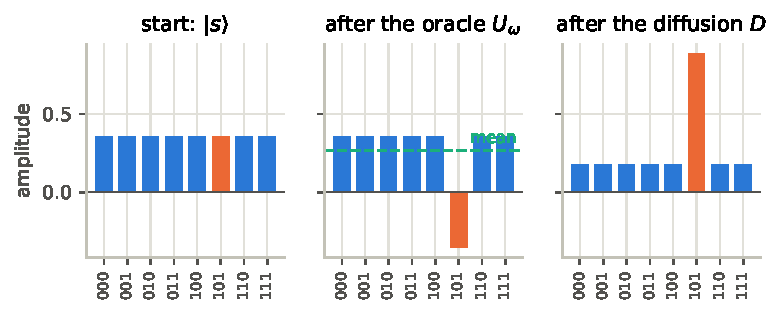
\includegraphics[width=0.84\textwidth]{amp_steps_n3}\\[0mm]
  \raggedright
  With $a = 1/\sqrt8$: oracle gives seven $+a$ and one $-a$, with mean $\bar c = \frac{6a}{8} = \frac34a$.\\
  Diffusion: unmarked $2\cdot\frac34a - a = \frac12a$; marked $2\cdot\frac34a + a = \frac52a$. So $P_1 = \frac{25}{4}a^2 = \frac{25}{32} = 0.781$.
\end{frame}

\begin{frame}{Checking the numbers with CUDA-Q: $N = 8$}
  \begin{columns}[c]
    \begin{column}{0.58\textwidth}
      \centering\footnotesize
      \begin{tabular}{lrrr}
        \toprule
        after & unmarked $c_x$ & marked $c_x$ & $P(\text{marked})$\\
        \midrule
        \nthreerows
        \bottomrule
      \end{tabular}
    \end{column}
    \begin{column}{0.38\textwidth}
      \begin{itemize}
        \item Simulated with \texttt{cudaq.get\_state}.
        \item $0.3536 = a$, $\ 0.8839 = \frac52a$, $\ 0.9723 = \frac{11}{4}a$.
        \item $0.7812 = \frac{25}{32}$, $\ 0.9453 = \frac{121}{128}$.
      \end{itemize}
    \end{column}
  \end{columns}
  \vspace{3mm}
  \small The second diffusion by hand: the marked value is $-\frac52a$, the mean is $\frac{7\cdot\frac12a - \frac52a}{8} = \frac a8$, so marked $\to \frac a4 + \frac52a = \frac{11}{4}a$ and unmarked $\to \frac a4 - \frac12a = -\frac a4$.
  The unmarked amplitudes have \key{gone negative}: the mean is shrinking and the next step will overshoot.
\end{frame}

\begin{frame}{Too many iterations: over-rotation appears}
  \centering
  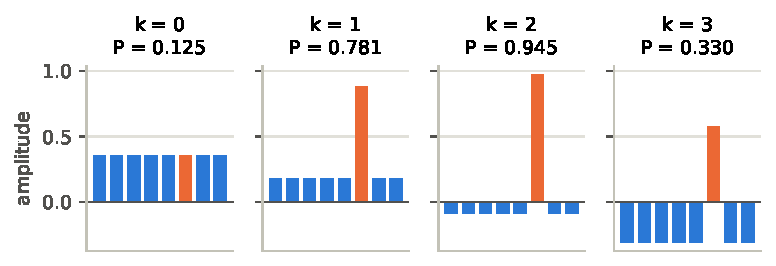
\includegraphics[width=0.9\textwidth]{amp_k_n3}\\[1mm]
  \raggedright
  CUDA-Q amplitudes for $N = 8$ (marked item in orange; overall sign removed).
  \begin{itemize}
    \item $k = 2$ is the best choice: $P = 0.945$.
    \item At $k = 3$ the probability has dropped to $0.330$: the search \hl{overshoots}.
    \item Unlike a classical search, you cannot simply run ``a bit longer to be safe''.
  \end{itemize}
\end{frame}

\begin{frame}[fragile]{The algorithm as pseudocode}
  \begin{columns}[T]
    \begin{column}{0.55\textwidth}
\begin{lstlisting}[language={}]
input : oracle for f on n qubits, number M >= 1
output: a marked item, with high probability

theta = arcsin( sqrt(M / 2^n) )
k     = round( pi / (4 * theta) - 1/2 )

prepare |0...0>
apply H to every qubit          # |s>
repeat k times:
    apply oracle U_omega        # flip marked signs
    apply diffusion D           # invert about mean
measure all qubits -> x
if f(x) == 1: return x          # one classical check
else: run again
\end{lstlisting}
    \end{column}
    \begin{column}{0.41\textwidth}
      \begin{block}{Why the last check?}
        Success is probabilistic. A failed run is detected with one more use of $f$, and you repeat.
      \end{block}
      \vspace{1mm}
      The rest of this lecture explains where the formulas for $\theta$ and $k$ come from, and how to build the two blocks.
    \end{column}
  \end{columns}
\end{frame}

% =====================================================================================
\section{Part 5: The geometric picture and derivations}
\begin{frame}{Everything happens in a plane}
  Define the two normalised states
  \[ \ket{m} = \frac{1}{\sqrt M}\sum_{x\ \text{marked}}\ket{x}, \qquad \ket{r} = \frac{1}{\sqrt{N - M}}\sum_{x\ \text{unmarked}}\ket{x}. \]
  They are orthogonal, and the start state is a combination of them:
  \begin{block}{Start state in the plane}
    \[ \ket{s} = \sqrt{\frac{N - M}{N}}\,\ket{r} + \sqrt{\frac MN}\,\ket{m} = \cos\theta\,\ket{r} + \sin\theta\,\ket{m}, \qquad \sin\theta = \sqrt{\frac MN} \]
  \end{block}
  \begin{itemize}
    \item $\theta$ is the angle between $\ket{s}$ and the unmarked axis. Example: $N = 16$, $M = 1$: $\sin\theta = \frac14$, $\theta = 14.5^\circ$.
    \item Both $\Uo$ and $D$ map this plane to itself, so we can forget the other $N - 2$ dimensions.
  \end{itemize}
\end{frame}

\begin{frame}{The oracle and the diffusion are reflections}
  \centering
  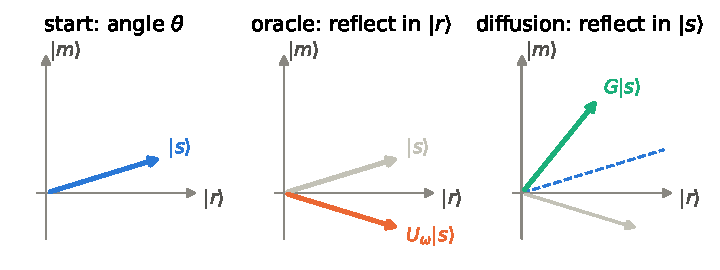
\includegraphics[width=0.84\textwidth]{geometry_steps}\\
  \raggedright
  \begin{itemize}
    \item $\Uo$: fixes $\ket{r}$, negates $\ket{m}$. That is the \key{reflection in the line through $\ket{r}$} (angle $0$).
    \item $D$: fixes $\ket{s}$, negates the perpendicular direction. That is the \key{reflection in the line through $\ket{s}$} (angle $\theta$).
    \item Two reflections with lines $\theta$ apart: a \hl{rotation by $2\theta$} towards $\ket{m}$.
  \end{itemize}
\end{frame}

\begin{frame}{The Grover operator as a matrix}
  \begin{columns}[T]
    \begin{column}{0.56\textwidth}
      In the basis $\{\ket{r}, \ket{m}\}$:
      \[ \Uo = \begin{pmatrix}1&0\\0&-1\end{pmatrix}, \]
      \[ \ket{s} = \begin{pmatrix}\cos\theta\\ \sin\theta\end{pmatrix}, \quad D = \begin{pmatrix}\cos2\theta & \sin2\theta\\ \sin2\theta & -\cos2\theta\end{pmatrix}. \]
      Multiplying ($2\cos^2\theta - 1 = \cos2\theta$, $\ 2\sin\theta\cos\theta = \sin2\theta$):
      \begin{block}{Rotation by $2\theta$}
        \[ G = D\Uo = \begin{pmatrix}\cos2\theta & -\sin2\theta\\ \sin2\theta & \cos2\theta\end{pmatrix} \]
      \end{block}
    \end{column}
    \begin{column}{0.4\textwidth}
      \begin{exampleblock}{Eigenvalues}
        A rotation by $2\theta$ has eigenvalues $e^{\pm2i\theta}$ and eigenvectors
        \[ \tfrac{1}{\sqrt2}\big(\ket{r} \mp i\ket{m}\big). \]
        $N = 16$, $M = 1$: $\cos2\theta = \frac78$, $\ \sin2\theta = \frac{\sqrt{15}}{8}$; eigenvalues $\frac{7 \pm i\sqrt{15}}{8}$.
      \end{exampleblock}
      \small Quantum counting will read $\theta$ from these eigenvalues.
    \end{column}
  \end{columns}
\end{frame}

\begin{frame}{Deriving the success probability}
  \begin{columns}[c]
    \begin{column}{0.58\textwidth}
      $\ket{s}$ sits at angle $\theta$, and each $G$ adds $2\theta$. After $k$ iterations the angle is $\theta + 2k\theta = (2k + 1)\theta$:
      \begin{block}{State after $k$ iterations}
        \[ G^k\ket{s} = \sin\big((2k{+}1)\theta\big)\ket{m} + \cos\big((2k{+}1)\theta\big)\ket{r} \]
      \end{block}
      Measuring gives a marked item with probability $|\text{coefficient of }\ket{m}|^2$:
      \begin{alertblock}{Success probability}
        \[ P_k = \sin^2\big((2k + 1)\theta\big) \]
      \end{alertblock}
    \end{column}
    \begin{column}{0.38\textwidth}
      \centering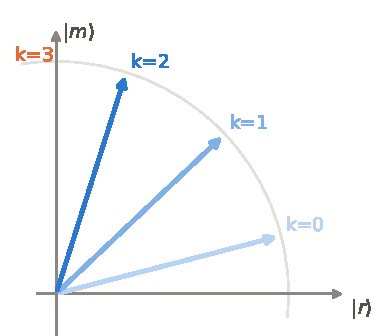
\includegraphics[width=\textwidth]{geometry_k_n4}\\
      \small $N = 16$: $\theta = 14.5^\circ$; the angles are $14.5^\circ$, $43.4^\circ$, $72.4^\circ$, $101.3^\circ$. $k = 3$ passes just beyond $\ket{m}$.
    \end{column}
  \end{columns}
\end{frame}

\begin{frame}{Deriving the optimal number of iterations}
  We want $(2k + 1)\theta$ as close as possible to $\frac\pi2$:
  \[ (2k + 1)\theta = \frac\pi2 \quad\Longrightarrow\quad k = \frac{\pi}{4\theta} - \frac12 . \]
  \begin{block}{Optimal number of iterations}
    \[ \kopt = \mathrm{round}\Big(\frac{\pi}{4\theta} - \frac12\Big) \approx \frac\pi4\sqrt{\frac NM} \qquad (\text{using } \theta \approx \sqrt{M/N} \text{ for } M \ll N) \]
  \end{block}
  \begin{columns}[T]
    \begin{column}{0.5\textwidth}
      \key{Bound}: rounding leaves the angle within $\theta$ of $\frac\pi2$, so
      \[ P_{\kopt} \ge \cos^2\theta = 1 - \frac MN. \]
    \end{column}
    \begin{column}{0.46\textwidth}
      \begin{alertblock}{Finite-size trap}
        $n = 8$: $\frac\pi4\sqrt{256} = 12.57$ rounds to 13, but the exact rule gives $12.06 \to 12$. $P_{12} = 0.99995$, $\ P_{13} = 0.986$.
      \end{alertblock}
    \end{column}
  \end{columns}
\end{frame}

\begin{frame}{Optimal iterations in numbers}
  \begin{columns}[c]
    \begin{column}{0.55\textwidth}
      \centering\small
      \begin{tabular}{rrrrr}
        \toprule
        $n$ & $N$ & $\theta$ (rad) & $\kopt$ & $P$\\
        \midrule
        2 & 4 & 0.5236 & 1 & 1.0000\\
        3 & 8 & 0.3614 & 2 & 0.9453\\
        4 & 16 & 0.2527 & 3 & 0.9613\\
        5 & 32 & 0.1777 & 4 & 0.9992\\
        6 & 64 & 0.1253 & 6 & 0.9966\\
        8 & 256 & 0.0625 & 12 & 0.9999\\
        10 & 1\,024 & 0.0313 & 25 & 0.9995\\
        15 & 32\,768 & 0.0055 & 142 & 1.0000\\
        20 & 1\,048\,576 & 0.00098 & 804 & 1.0000\\
        \bottomrule
      \end{tabular}
    \end{column}
    \begin{column}{0.42\textwidth}
      \centering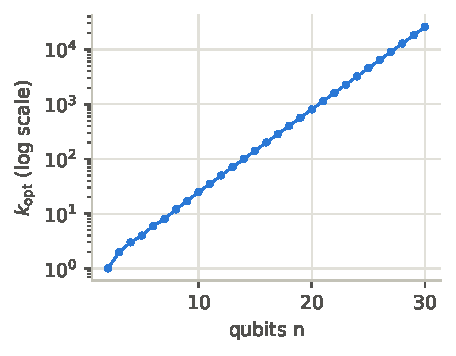
\includegraphics[width=0.92\textwidth]{kopt_scaling}\\
      \raggedright\small
      Optimal does not mean perfect: $P$ is usually slightly below 1. Each extra qubit multiplies $\kopt$ by about $\sqrt2$, so a straight line on the log scale.
    \end{column}
  \end{columns}
\end{frame}

\begin{frame}{Over-rotation: more is not better}
  \centering
  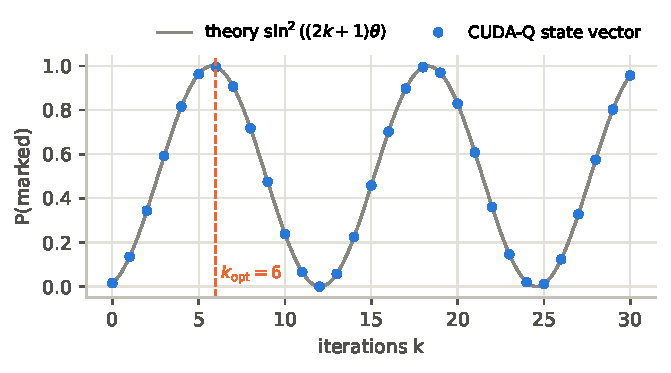
\includegraphics[width=0.74\textwidth]{p_vs_k_n6}\\[0mm]
  \raggedright
  $n = 6$, one marked item (CUDA-Q state vector, largest deviation from theory \devsix). After $k \approx \kopt$ the state rotates \key{past} $\ket{m}$; at $k \approx 2\kopt$ it is back near $\ket{r}$, and the marked item is \hl{less} likely than a random guess. One full period lasts $\frac{\pi}{2\theta}$ iterations.
\end{frame}

\begin{frame}{Complexity: Grover against classical search}
  \begin{columns}[T]
    \begin{column}{0.56\textwidth}
      \centering\small
      \begin{tabular}{lcc}
        \toprule
        & classical & quantum\\
        \midrule
        queries (one solution) & $\frac N2$ average & $\frac\pi4\sqrt N$\\
        queries ($M$ solutions) & $\Theta(N/M)$ & $\Theta(\sqrt{N/M})$\\
        lower bound & $\Omega(N/M)$ & $\Omega(\sqrt{N/M})$\\
        memory & small & $n$ qubits\\
        \bottomrule
      \end{tabular}\\[3mm]
      \raggedright\normalsize
      The ratio of queries is $\frac{N/2}{(\pi/4)\sqrt N} = \frac2\pi\sqrt N$. For $n = 20$: $652$ times fewer queries.
    \end{column}
    \begin{column}{0.4\textwidth}
      \begin{block}{Optimality}
        Bennett, Bernstein, Brassard and Vazirani: \emph{any} black-box quantum search needs $\Omega(\sqrt N)$ queries. Zalka: $\frac\pi4\sqrt N$ is optimal, including the constant.
      \end{block}
    \end{column}
  \end{columns}
\end{frame}

\begin{frame}{Why quadratic and not exponential?}
  \begin{columns}[T]
    \begin{column}{0.5\textwidth}
      \begin{itemize}
        \item One iteration rotates by only $2\theta \approx 2/\sqrt N$. We must travel about $\frac\pi2$, so about $\sqrt N$ steps are needed.
        \item The lower bound shows that no cleverness can beat this in the black-box model.
        \item $2^{n/2}$ is still \hl{exponential in $n$}. Grover does not make NP-complete problems easy.
      \end{itemize}
    \end{column}
    \begin{column}{0.46\textwidth}
      \begin{alertblock}{Theory versus practice}
        \key{Theory} counts queries.\\[1mm]
        \key{Practice} counts gates and time: each query runs the whole oracle circuit, with error correction on real hardware. The constant factors can absorb much of a quadratic gain.
      \end{alertblock}
    \end{column}
  \end{columns}
\end{frame}

\begin{frame}{Several marked items}
  \begin{columns}[c]
    \begin{column}{0.46\textwidth}
      Only the angle changes:
      \[ \sin\theta = \sqrt{M/N}, \quad \kopt \approx \frac\pi4\sqrt{N/M}. \]
      The final state is the uniform superposition of the solutions, so a measurement returns a random solution.
      \begin{exampleblock}{Worked example}
        $N = 1024$, $M = 16$: $\sin\theta = \frac18$, $\frac{\pi}{4\theta} - \frac12 = 5.77$, so $k = 6$ and $P = 0.9966$.
      \end{exampleblock}
    \end{column}
    \begin{column}{0.5\textwidth}
      \centering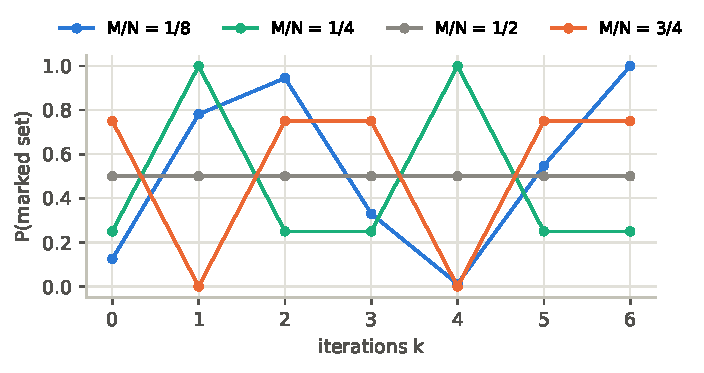
\includegraphics[width=\textwidth]{ratios}\\
      \raggedright\small
      Theory curves. $M/N = \frac14$: one step is exact. $\frac12$: flat at $\frac12$. $\frac34$: one step erases all marked weight ($P_1 = 0$). If $M > N/2$, just measure. \hl{Note:} the notebook handles one marked item only.
    \end{column}
  \end{columns}
\end{frame}

\begin{frame}[fragile]{Worked example: two marked items, $N = 8$}
  \begin{columns}[T]
    \begin{column}{0.5\textwidth}
      Marked: $\ket{101}$ and $\ket{110}$. Let $a = 1/\sqrt8$.
      \begin{enumerate}
        \item Oracle: six $+a$, two $-a$. Mean $\bar c = \frac{4a}{8} = \frac a2$.
        \item Diffusion: unmarked $2\bar c - a = 0$; marked $2\bar c + a = 2a$.
        \item Total probability: $2\times(2a)^2 = 8a^2 = 1$.
      \end{enumerate}
      \begin{block}{Check}
        $\sin^2\theta = \frac28 = \frac14$, so $\theta = 30^\circ$ and $P_1 = \sin^2 90^\circ = 1$.
      \end{block}
      Final state $\frac{1}{\sqrt2}(\ket{101} + \ket{110})$: each solution with probability $\frac12$.
    \end{column}
    \begin{column}{0.46\textwidth}
      \centering
      \begin{quantikz}[row sep=0.4cm, column sep=0.36cm]
        \lstick{$q_1$} & \qw & \ctrl{1} & \qw & \qw & \ctrl{1} & \qw & \qw\\
        \lstick{$q_2$} & \gate{X} & \ctrl{1} & \gate{X} & \qw & \ctrl{1} & \qw & \qw\\
        \lstick{$q_3$} & \qw & \control{} & \qw & \gate{X} & \control{} & \gate{X} & \qw
      \end{quantikz}\\[2mm]
      \small One oracle per marked string, one after the other; diagonal matrices just multiply their signs.\\[1mm]
      \hl{Theory only}: \texttt{Grover.ipynb} marks exactly one string.
    \end{column}
  \end{columns}
\end{frame}

\begin{frame}{Unknown number of solutions}
  \begin{columns}[c]
    \begin{column}{0.52\textwidth}
      Choosing $k$ needs $M$. If $M$ is unknown, a fixed $k$ may overshoot. \key{BBHT} (Boyer, Brassard, H{\o}yer, Tapp) uses a random $k$:
      \begin{block}{Average success}
        \[ \frac1m\sum_{k=0}^{m-1}\sin^2((2k{+}1)\theta) = \frac12 - \frac{\sin4m\theta}{4m\sin2\theta} \]
        This is at least $\frac14$ once $m \ge 1/\sin2\theta$.
      \end{block}
      \small Start with $m = 1$; pick $k$ below $m$; measure and check; if it fails, grow $m$ by a factor such as $\frac65$. Expected queries: $O(\sqrt{N/M})$.
    \end{column}
    \begin{column}{0.44\textwidth}
      \centering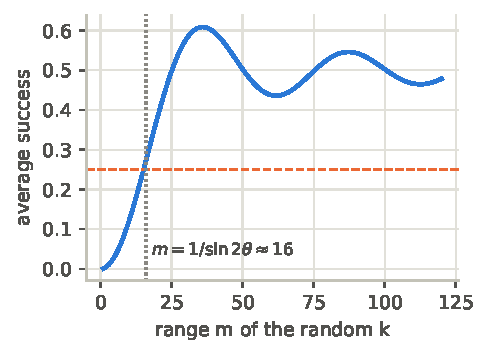
\includegraphics[width=\textwidth]{bbht_average}\\
      \small $n = 10$, $M = 1$: above $m \approx 16$ the average never falls below $\frac14$ (dashed), and it settles at $\frac12$.
    \end{column}
  \end{columns}
\end{frame}

\begin{frame}{Exact and fixed-point search}
  \begin{columns}[T]
    \begin{column}{0.48\textwidth}
      \begin{block}{Exact amplitude amplification}
        $P_{\kopt}$ can miss 1. Fix: round $k$ \hl{up}, then shrink the angle a little so that it lands exactly on $\frac\pi2$:
        \[ \theta' = \frac{\pi}{2(2k + 1)} \le \theta. \]
        Example $N = 16$: $k = 3$, $\ \theta' = \frac{\pi}{14} = 0.224 < 0.253$.\\[1mm]
        A smaller marked weight (an extra ancilla rotation) gives $P = 1$.
      \end{block}
    \end{column}
    \begin{column}{0.48\textwidth}
      \begin{block}{Fixed-point search}
        Grover's $\pi/3$ method uses reflections with phase $\frac\pi3$. One recursion turns the failure probability $\varepsilon$ into $\varepsilon^3$; extra steps cannot over-rotate.\\[1mm]
        Example: $0.2 \to 0.008 \to 5.12\times10^{-7}$. The basic form gives up the quadratic speed-up; later variants recover it.
      \end{block}
    \end{column}
  \end{columns}
  \vspace{2mm}
  \small \key{Maximum success is not minimum cost.} Repeat-until-success costs $k/P_k$ queries: $N = 16$ gives $2.12$, $2.20$, $3.12$ for $k = 1, 2, 3$, so the cheapest is $k = 1$, not $\kopt = 3$.
\end{frame}

\begin{frame}{Amplitude amplification in general}
  Grover's trick works for \key{any} procedure $\mathcal{A}$ (with no measurements) that succeeds with probability $a$.
  \begin{block}{Amplitude amplification (Brassard, H{\o}yer, Mosca, Tapp)}
    \[ Q = -\mathcal{A}S_0\mathcal{A}^{-1}S_\chi, \qquad \sin^2\theta = a, \qquad P_k = \sin^2\big((2k+1)\theta\big) \]
  \end{block}
  \begin{columns}[T]
    \begin{column}{0.5\textwidth}
      \begin{itemize}
        \item $S_\chi$ flips the sign of good states; $S_0 = I - 2\pj{0}$.
        \item Grover is the case $\mathcal{A} = H^{\otimes n}$, $\ a = M/N$.
        \item Uses of $\mathcal{A}$ or $\mathcal{A}^{-1}$: $2k + 1$.
      \end{itemize}
    \end{column}
    \begin{column}{0.46\textwidth}
      \begin{exampleblock}{Worked example}
        $a = 0.04$: $\theta = 0.2014$, $\ k = 3$, $\ 7$ uses of $\mathcal{A}$, $\ P = 0.974$. Classical repetition needs 25 runs on average.
      \end{exampleblock}
    \end{column}
  \end{columns}
\end{frame}

\begin{frame}{Quantum counting: finding $M$}
  \begin{columns}[c]
    \begin{column}{0.45\textwidth}
      Run \key{phase estimation} on $G$, starting from $\ket{s}$, an equal mix of both eigenvectors. With $e^{2\pi i\varphi} = e^{\pm2i\theta}$:
      \[ \varphi = \frac\theta\pi \ \text{ or }\ 1 - \frac\theta\pi. \]
      Outcome $y$ on $t$ counting qubits:
      \[ \tilde\theta = \frac{\pi y}{2^t}, \quad \tilde M = N\sin^2\tilde\theta. \]
    \end{column}
    \begin{column}{0.52\textwidth}
      \centering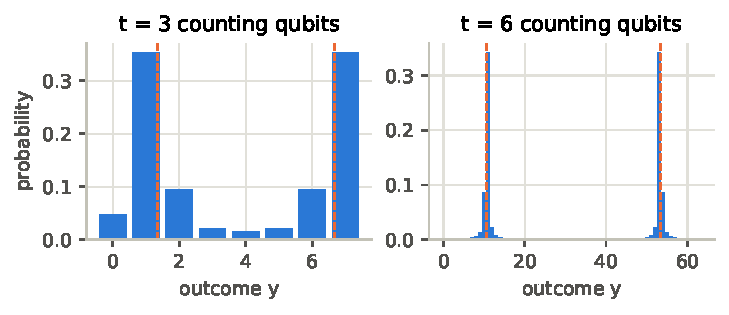
\includegraphics[width=\textwidth]{counting}\\
      \raggedright\small
      $N = 64$, $M = 16$ (theory, explicit matrices), so $\varphi = \frac16, \frac56$ (dashed). $t = 3$: the likely $y = 1$ gives $\tilde M \approx 9.4$, and $y = 2$ gives $32$: too coarse. $t = 6$: peaks at $y = 11$ and $53$ give $\tilde M \approx 16.9$. More qubits give finer estimates.
    \end{column}
  \end{columns}
\end{frame}

% =====================================================================================
\section{Part 6: Building the circuit}
\begin{frame}[fragile]{The oracle circuit}
  \begin{columns}[c]
    \begin{column}{0.42\textwidth}
      \centering
      \begin{quantikz}[row sep=0.42cm, column sep=0.5cm]
        \lstick{$q_1$} & \qw & \ctrl{1} & \qw & \qw\\
        \lstick{$q_2$} & \gate{X} & \ctrl{1} & \gate{X} & \qw\\
        \lstick{$q_3$} & \qw & \control{} & \qw & \qw
      \end{quantikz}\\[2mm]
      \small Oracle for $\ket{\xs} = \ket{101}$
    \end{column}
    \begin{column}{0.54\textwidth}
      \begin{block}{Recipe (no ancillas)}
        \begin{enumerate}
          \item $X$ on every qubit where $\xs$ has a 0
          \item multi-controlled $Z$ on all $n$ qubits
          \item the same $X$ gates again
        \end{enumerate}
      \end{block}
      Result: $\Uo = I - 2\pj{\xs}$.\\[1mm]
      Gates: $2z + 1$, with $z$ the number of zeros in $\xs$.\\[1mm]
      \small This is a \hl{demonstration oracle}: it contains the answer. A real oracle would compute $f$ from the problem, and is the expensive part.
    \end{column}
  \end{columns}
\end{frame}

\begin{frame}[fragile]{The diffusion circuit}
  \begin{columns}[c]
    \begin{column}{0.48\textwidth}
      \centering
      \begin{quantikz}[row sep=0.42cm, column sep=0.42cm]
        \lstick{$q_1$} & \gate{H} & \gate{X} & \ctrl{1} & \gate{X} & \gate{H} & \qw\\
        \lstick{$q_2$} & \gate{H} & \gate{X} & \ctrl{1} & \gate{X} & \gate{H} & \qw\\
        \lstick{$q_3$} & \gate{H} & \gate{X} & \control{} & \gate{X} & \gate{H} & \qw
      \end{quantikz}
    \end{column}
    \begin{column}{0.48\textwidth}
      Read the middle first, using the conjugation rule:
      \[ \mathrm{C}^{n-1}\mathrm{Z} = I - 2\pj{1\dots1} \]
      \[ \xrightarrow{X^{\otimes n}}\ I - 2\pj{0\dots0} \]
      \[ \xrightarrow{H^{\otimes n}}\ I - 2\pj{s} = -D \]
      Gates: $4n + 1$.
    \end{column}
  \end{columns}
  \vspace{3mm}
  \begin{alertblock}{The minus sign}
    The circuit implements $-D$, not $D$. The factor $-1$ is a \hl{global phase}: it has no observable effect. It is why simulators may show every amplitude with the opposite sign.
  \end{alertblock}
\end{frame}

\begin{frame}[fragile]{The two-qubit Grover circuit, $\ket{\xs} = \ket{10}$}
  \centering
  \begin{quantikz}[row sep=0.5cm, column sep=0.4cm]
    \lstick{$\ket0$} & \gate{H} & \qw & \ctrl{1} & \qw & \gate{H} & \gate{X} & \ctrl{1} & \gate{X} & \gate{H} & \meter{}\\
    \lstick{$\ket0$} & \gate{H} & \gate{X} & \control{} & \gate{X} & \gate{H} & \gate{X} & \control{} & \gate{X} & \gate{H} & \meter{}
  \end{quantikz}\\[3mm]
  \raggedright
  \begin{columns}[T]
    \begin{column}{0.48\textwidth}
      \begin{itemize}
        \item $n = 2$, so $\theta = 30^\circ$ and $\kopt = 1$.
        \item With two qubits, the multi-controlled $Z$ is the ordinary CZ.
        \item Marked string $10$ has one zero, on qubit 2.
      \end{itemize}
    \end{column}
    \begin{column}{0.48\textwidth}
      \begin{block}{Gate count}
        $H$ layer: 2. Oracle: $2 + 1 = 3$. Diffusion: $8 + 1 = 9$. Total $14$ gates; formula $n + k(4n + 2z + 2) = 2 + 12$.
      \end{block}
    \end{column}
  \end{columns}
\end{frame}

\begin{frame}{Step-by-step execution of the two-qubit circuit}
  Amplitudes of $(\ket{00}, \ket{01}, \ket{10}, \ket{11})$, multiplied by 2 for readability:\\[2mm]
  \centering\small
  \begin{tabular}{llr}
    \toprule
    block & after gate & $2\times$ amplitudes\\
    \midrule
    start & $\ket{00}$ & $(2, 0, 0, 0)$\\
    preparation & $H \otimes H$ & $(1, 1, 1, 1)$\\
    \midrule
    oracle & $X$ on $q_2$ & $(1, 1, 1, 1)$\\
    & CZ & $(1, 1, 1, -1)$\\
    & $X$ on $q_2$ & $(1, 1, -1, 1)$\\
    \midrule
    diffusion & $H \otimes H$ & $(1, -1, 1, 1)$\\
    & $X \otimes X$ & $(1, 1, -1, 1)$\\
    & CZ & $(1, 1, -1, -1)$\\
    & $X \otimes X$ & $(-1, -1, 1, 1)$\\
    & $H \otimes H$ & $(0, 0, -2, 0)$\\
    \bottomrule
  \end{tabular}\\[2mm]
  \raggedright\normalsize
  The final state is $-\ket{10}$: measuring returns $10$ with probability 1. The minus sign is the global phase from $-D$.
\end{frame}

\begin{frame}[fragile]{The three-qubit Grover circuit, $\ket{\xs} = \ket{101}$}
  \centering
  \begin{quantikz}[row sep=0.42cm, column sep=0.3cm]
    \lstick{$\ket0$} & \gate{H} & \qw & \ctrl{1} & \qw & \gate{H} & \gate{X} & \ctrl{1} & \gate{X} & \gate{H} & \ \cdots\ & \meter{}\\
    \lstick{$\ket0$} & \gate{H} & \gate{X} & \ctrl{1} & \gate{X} & \gate{H} & \gate{X} & \ctrl{1} & \gate{X} & \gate{H} & \ \cdots\ & \meter{}\\
    \lstick{$\ket0$} & \gate{H} & \qw & \control{} & \qw & \gate{H} & \gate{X} & \control{} & \gate{X} & \gate{H} & \ \cdots\ & \meter{}
  \end{quantikz}\\[3mm]
  \raggedright
  \begin{itemize}
    \item Oracle: the columns $X_2$, CCZ, $X_2$. Diffusion: the next five columns. The dots mean ``repeat the two blocks''.
    \item $\kopt = 2$ iterations: $\frac{\pi}{4\theta} - \frac12 = 1.67 \to 2$. Gates: $3 + 2\times(12 + 2 + 2) = 35$.
    \item Probabilities: $P_0 = \frac18$, $\ P_1 = \frac{25}{32}$, $\ P_2 = \frac{121}{128}$. A third iteration would give only $0.330$.
  \end{itemize}
\end{frame}

\begin{frame}[fragile]{The four-qubit Grover circuit, $\ket{\xs} = \ket{1011}$}
  \centering
  \begin{quantikz}[row sep=0.3cm, column sep=0.3cm]
    \lstick{$\ket0$} & \gate{H} & \qw & \ctrl{1} & \qw & \gate{H} & \gate{X} & \ctrl{1} & \gate{X} & \gate{H} & \ \cdots\ & \meter{}\\
    \lstick{$\ket0$} & \gate{H} & \gate{X} & \ctrl{1} & \gate{X} & \gate{H} & \gate{X} & \ctrl{1} & \gate{X} & \gate{H} & \ \cdots\ & \meter{}\\
    \lstick{$\ket0$} & \gate{H} & \qw & \ctrl{1} & \qw & \gate{H} & \gate{X} & \ctrl{1} & \gate{X} & \gate{H} & \ \cdots\ & \meter{}\\
    \lstick{$\ket0$} & \gate{H} & \qw & \control{} & \qw & \gate{H} & \gate{X} & \control{} & \gate{X} & \gate{H} & \ \cdots\ & \meter{}
  \end{quantikz}\\[2mm]
  \raggedright
  \begin{itemize}
    \item One zero in $\xs$, so one $X$ pair in the oracle. Now the multi-controlled $Z$ has 3 controls.
    \item $\kopt = 3$: gates $4 + 3\times(16 + 2 + 2) = 64$, plus 4 measurements. $\ P_3 = 0.9613$.
  \end{itemize}
\end{frame}

\begin{frame}{Measurement outcomes: four qubits with CUDA-Q}
  \centering
  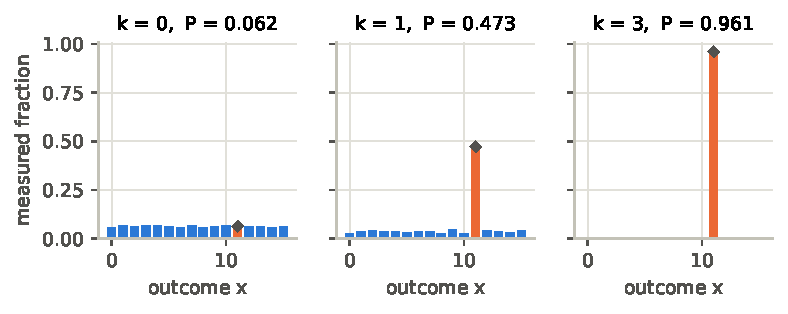
\includegraphics[width=0.84\textwidth]{shots_n4}\\[0mm]
  \raggedright
  \begin{columns}[c]
    \begin{column}{0.46\textwidth}
      \centering\small
      \begin{tabular}{crrr}
        \toprule
        $k$ & theory $P_k$ & counts & fraction\\
        \midrule
        \shotsrows
        \bottomrule
      \end{tabular}
    \end{column}
    \begin{column}{0.5\textwidth}
      \small 2000 shots each; orange marks $\ket{1011}$, the diamond the theory value. Binomial spread: $\sqrt{SP(1 - P)}$. At $k = 3$: $\sqrt{2000\times0.961\times0.039} \approx 9$ counts.
    \end{column}
  \end{columns}
\end{frame}

\begin{frame}{Gate count and circuit depth}
  \begin{columns}[T]
    \begin{column}{0.5\textwidth}
      With $z$ zeros in $\xs$, one iteration has:
      \begin{itemize}
        \item $2n$ Hadamards
        \item $2n + 2z$ $X$ gates
        \item 2 multi-controlled $Z$ gates
      \end{itemize}
      \begin{block}{Total}
        $n + k(4n + 2z + 2)$ gates, plus $n$ measurements. Depth: $2 + 8k$ layers.
      \end{block}
    \end{column}
    \begin{column}{0.46\textwidth}
      \begin{exampleblock}{Notebook default: $n = 15$, $k = 142$, $z = 6$}
        \begin{itemize}
          \item \texttt{h}: $15 + 142\times30 = 4275$
          \item \texttt{x}: $142\times42 = 5964$
          \item multi-controlled $Z$: $284$
          \item measurements: $15$
        \end{itemize}
        Total $10\,538$ operations and depth $1138$: exactly what the notebook reports.
      \end{exampleblock}
    \end{column}
  \end{columns}
\end{frame}

\begin{frame}[fragile]{Ancillas and circuit decomposition}
  \begin{columns}[c]
    \begin{column}{0.5\textwidth}
      A simulator applies C$^{n-1}$Z directly. Hardware cannot: it must be \key{decomposed} into one- and two-qubit gates.
      \begin{block}{Textbook construction}
        A multi-controlled $Z$ with $m$ controls uses $m - 1$ clean \key{ancillas}, $2(m - 1)$ Toffoli gates and one CZ.
      \end{block}
      Example: $n = 10$, $m = 9$: 16 Toffolis per gate, so 32 per iteration.
    \end{column}
    \begin{column}{0.46\textwidth}
      \centering
      \begin{quantikz}[row sep=0.22cm, column sep=0.3cm]
        \lstick{$c_1$} & \ctrl{1} & \qw & \qw & \qw & \ctrl{1} & \qw\\
        \lstick{$c_2$} & \ctrl{2} & \qw & \qw & \qw & \ctrl{2} & \qw\\
        \lstick{$c_3$} & \qw & \ctrl{1} & \qw & \ctrl{1} & \qw & \qw\\
        \lstick{$\ket0$} & \targ{} & \ctrl{1} & \qw & \ctrl{1} & \targ{} & \qw\\
        \lstick{$\ket0$} & \qw & \targ{} & \ctrl{1} & \targ{} & \qw & \qw\\
        \lstick{$t$} & \qw & \qw & \control{} & \qw & \qw & \qw
      \end{quantikz}\\[1mm]
      \small $m = 3$: compute into two ancillas (4 Toffolis in all), apply one CZ, uncompute. \hl{The repository's notebook uses no ancillas}: it calls \texttt{z.ctrl} directly.
    \end{column}
  \end{columns}
\end{frame}

% =====================================================================================
\section{Part 7: Implementation and results}
\begin{frame}{The notebook: \texttt{Grover.ipynb}}
  \begin{columns}[T]
    \begin{column}{0.5\textwidth}
      \begin{block}{What it does}
        Search for \hl{exactly one} marked bit string, with the oracle built from $X$ gates and \texttt{z.ctrl}.
      \end{block}
      \small
      \begin{tabular}{ll}
        \toprule
        section & content\\
        \midrule
        1 & problem and mathematics\\
        3 & input parameters (edit only this)\\
        4 & validates inputs; $\theta$, $k_{\rm opt}$\\
        6 & expected result, memory, time\\
        7 & kernels and circuit drawing\\
        8 & execution with memory monitor\\
        9, 10 & plots and benchmark report\\
        \bottomrule
      \end{tabular}
    \end{column}
    \begin{column}{0.46\textwidth}
      \begin{exampleblock}{Default input (Section 3)}
        \small
        \texttt{N\_QUBITS = 15}\\
        \texttt{MARKED\_BITSTRING = "example"}\\
        \texttt{GROVER\_ITERATIONS = "optimal"}\\
        \texttt{RUN\_ITERATION\_SWEEP = True}\\
        \texttt{SHOTS = 2000}\\
        \texttt{BACKEND = "auto"}\\
        \texttt{SIMULATION\_METHOD = "statevector"}
      \end{exampleblock}
      \small Notebook source: \texttt{build\_grover.py} in \texttt{dev/notebook\_builders/}. Results go to \texttt{exports/grover/}.
    \end{column}
  \end{columns}
\end{frame}

\begin{frame}{From formula to code}
  \centering\footnotesize
  \begin{tabular}{lll}
    \toprule
    mathematics & in \texttt{build\_grover.py} & note\\
    \midrule
    $N$ items & \texttt{search\_space = 2 ** N\_QUBITS} & notebook: $M$\\
    $\sin\theta = 1/\sqrt N$ & \texttt{theta = math.asin(1.0 / math.sqrt(search\_space))} & one marked\\
    $k_{\rm opt}$ & \texttt{max(0, round(math.pi / (4 * theta) - 0.5))} & exact rule\\
    $\ket{s}$ & \texttt{h(qubits)} & all qubits\\
    $\Uo$ & \texttt{x}, \texttt{z.ctrl}, \texttt{x} & oracle\\
    $-D$ & \texttt{h, x, z.ctrl, x, h} & diffusion\\
    $P_k$ & \texttt{math.sin((2 * iterations + 1) * theta) ** 2} & theory\\
    $\sqrt{SP(1 - P)}$ & \texttt{math.sqrt(SHOTS * p\_theory * (1 - p\_theory))} & count spread\\
    \bottomrule
  \end{tabular}\\[3mm]
  \raggedright\normalsize
  Section 4 of the notebook checks the inputs and rejects invalid ones: \texttt{N\_QUBITS} must be at least 2, and a marked string must have exactly \texttt{N\_QUBITS} characters 0 or 1.
\end{frame}

\begin{frame}[fragile]{Oracle and diffusion in code}
  \begin{columns}[T]
    \begin{column}{0.6\textwidth}
\begin{lstlisting}
@cudaq.kernel
def grover_iteration(qubits: cudaq.qview,
                     marked: list[int]):
    n = qubits.size()
    # Oracle: multiply the amplitude of |x*> by -1
    for i in range(n):
        if marked[i] == 0:
            x(qubits[i])              # maps |x*> onto |11...1>
    z.ctrl(qubits[0:n - 1], qubits[n - 1])
    for i in range(n):
        if marked[i] == 0:
            x(qubits[i])              # undo the X gates
    # Diffusion D = 2|s><s| - I
    h(qubits)                         # |s> -> |00...0>
    x(qubits)                         # |00...0> -> |11...1>
    z.ctrl(qubits[0:n - 1], qubits[n - 1])
    x(qubits)                         # undo X
    h(qubits)                         # undo H (result: -D)
\end{lstlisting}
    \end{column}
    \begin{column}{0.37\textwidth}
      \small
      \begin{itemize}
        \item \texttt{marked} lists the bits of $\xs$, qubit 0 first.
        \item \texttt{z.ctrl(controls, target)}: the first $n - 1$ qubits control a $Z$ on the last: C$^{n-1}$Z.
        \item \texttt{h(qubits)} applies $H$ to the whole register.
        \item The oracle comes first in the code: $G = D\Uo$.
      \end{itemize}
    \end{column}
  \end{columns}
\end{frame}

\begin{frame}[fragile]{The search kernel, shots and results}
  \begin{columns}[T]
    \begin{column}{0.58\textwidth}
\begin{lstlisting}
@cudaq.kernel
def grover_search(n: int, marked: list[int],
                  iterations: int):
    qubits = cudaq.qvector(n)    # n qubits, all in |0>
    h(qubits)                    # uniform superposition |s>
    for _ in range(iterations):
        grover_iteration(qubits, marked)
    mz(qubits)                   # measure in the Z basis

# Execution cell (Section 8), simplified
counts = cudaq.sample(kernels["search"], N_QUBITS,
                      marked_bits, iterations,
                      shots_count=SHOTS)
measured_marked = counts.count(marked_bitstring)
p_measured = measured_marked / SHOTS
most_frequent = counts.most_probable()
\end{lstlisting}
    \end{column}
    \begin{column}{0.39\textwidth}
      \small
      \begin{block}{Expected output}
        \texttt{cudaq.sample} returns bit strings and their counts: for example \texttt{\{ 011001010011111:2000 \}}.
      \end{block}
      \begin{itemize}
        \item \texttt{count(...)}: shots that returned $\xs$
        \item \texttt{p\_measured}: estimates $P_k$; the error is about $1/\sqrt{\text{shots}}$ or less
        \item \texttt{most\_probable()}: the search result
      \end{itemize}
    \end{column}
  \end{columns}
\end{frame}

\begin{frame}[fragile]{The iteration sweep: state vector instead of shots}
  \begin{columns}[T]
    \begin{column}{0.58\textwidth}
\begin{lstlisting}
stride = max(1, math.ceil(sweep_max / SWEEP_MAX_POINTS))
state = cudaq.get_state(kernels["uniform"], N_QUBITS)
k_done = 0
sweep_iterations.append(0)
sweep_probabilities.append(
    abs(state.amplitude(marked_bits)) ** 2)
while k_done + stride <= sweep_max:
    state = cudaq.get_state(kernels["continue"], state,
                            marked_bits, stride)
    k_done += stride
    sweep_iterations.append(k_done)
    sweep_probabilities.append(
        abs(state.amplitude(marked_bits)) ** 2)
\end{lstlisting}
    \end{column}
    \begin{column}{0.39\textwidth}
      \small
      \begin{itemize}
        \item \texttt{get\_state}: exact amplitudes, no shot noise.
        \item The state is handed to the next kernel, so the sweep costs only \texttt{sweep\_max} iterations.
        \item $n = 15$: $\texttt{sweep\_max} = 285$ and $\texttt{stride} = \lceil285/60\rceil = 5$, so $1 + 57 = 58$ points, as recorded.
        \item Holding two states doubles the memory: $2\times2^{15}\times16$ bytes $= 1.05$ MB.
      \end{itemize}
    \end{column}
  \end{columns}
\end{frame}

\begin{frame}{Backends: what the notebook offers}
  \centering\small
  \begin{tabular}{llll}
    \toprule
    \texttt{BACKEND} & \texttt{SIMULATION\_METHOD} & CUDA-Q target & status here\\
    \midrule
    \texttt{cpu} & \texttt{statevector} & \texttt{qpp-cpu} & recorded and re-run\\
    \texttt{cpu} & \texttt{density\_matrix} & \texttt{density-matrix-cpu} & noise slide only\\
    \texttt{gpu} & \texttt{statevector} & \texttt{nvidia} & \hl{not run}\\
    \texttt{gpu} & \texttt{mps}, \texttt{tensornet} & \texttt{tensornet-mps}, \texttt{tensornet} & \hl{not run}\\
    \texttt{multi-gpu} & \texttt{statevector} & \texttt{nvidia} (\texttt{mgpu}, MPI) & \hl{not run}\\
    \texttt{hardware} & provider & for example \texttt{quantinuum} & \hl{not run}\\
    \bottomrule
  \end{tabular}\\[3mm]
  \raggedright\normalsize
  \begin{itemize}
    \item A Jupyter kernel is one process, so one GPU. For several GPUs: \texttt{jupyter nbconvert --to script Grover.ipynb}, set \texttt{BACKEND = "multi-gpu"}, then \texttt{mpiexec -np 4 python Grover.py}.
    \item \texttt{BACKEND = "hardware"} with \texttt{HARDWARE\_EMULATE = True} compiles for a provider and runs locally at no cost.
    \item The code supports these options; \key{these slides make no claim about their performance}.
  \end{itemize}
\end{frame}

\begin{frame}{Previously recorded result: 15 qubits}
  \centering
  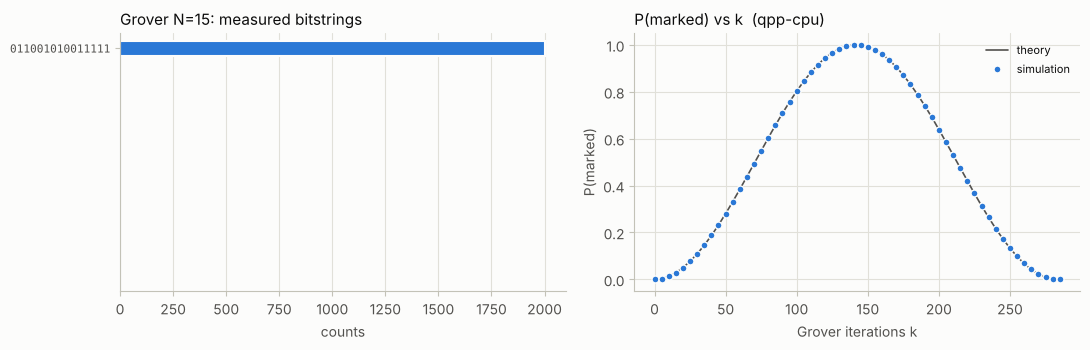
\includegraphics[width=0.8\textwidth]{notebook_run}\\[1mm]
  \raggedright\small
  \key{Stored output of \texttt{Grover.ipynb}} (CUDA-Q 0.16.0, \texttt{qpp-cpu}, 4 CPU cores, no GPU). Marked item \texttt{011001010011111}, $k = 142$: 2000 of 2000 shots correct. Sweep: 58 points, largest deviation from theory $8.2\times10^{-13}$.
  Times: execution 23.3\,s, sweep 43.3\,s, cell total 66.8\,s. Peak process memory 0.55\,GB.
\end{frame}

\begin{frame}[fragile]{Expected output, and what it means}
  \begin{columns}[T]
    \begin{column}{0.58\textwidth}
\begin{lstlisting}[language={},basicstyle=\ttfamily\scriptsize]
Grover iterations (k)   : 142 (optimal: 142)
Marked bitstring        : 011001010011111
Expected result         : P(marked) = 0.999987
Actual result           : P(marked) = 1.0000 (2000/2000)
Error |P_measured - P_theory| : 0.0000
1-sigma shot noise      : 0.0001
Sweep max deviation     : 8.20e-13
Search succeeded        : YES
Quantum execution time  : 23.3304 s
Iteration sweep time    : 43.3148 s
Peak process RSS        : 0.55 GB (baseline 0.53 GB)
\end{lstlisting}
      \small Excerpt of the stored benchmark report (Section 10); labels shortened to fit.
    \end{column}
    \begin{column}{0.39\textwidth}
      \small
      \begin{itemize}
        \item \key{Expected vs.\ actual}: theory from $\sin^2((2k+1)\theta)$; measurement from \texttt{counts}.
        \item \key{Shot noise}: $\sqrt{P(1-P)/S}$ is tiny here because $P \approx 1$.
        \item \key{Sweep deviation}: exact amplitudes against theory: only rounding error.
        \item \key{Time, memory}: true for that machine, that day. They are not part of the theory.
      \end{itemize}
    \end{column}
  \end{columns}
\end{frame}

\begin{frame}{Newly executed: the same circuit, and how to read it}
  \begin{columns}[T]
    \begin{column}{0.5\textwidth}
      \key{Re-run for these slides} (\hostinfo):
      \begin{itemize}
        \item Gates counted by CUDA-Q: \hcount{} \texttt{h}, \xcount{} \texttt{x}: identical to the notebook.
        \item Marked counts: \marksfifteen{} of 2000.
        \item Run time: \timefifteen\,s (one run).
      \end{itemize}
      \vspace{1mm}
      \small 2000/2000 and 1999/2000 are both consistent with the theory. They are different random samples.
    \end{column}
    \begin{column}{0.46\textwidth}
      \begin{exampleblock}{How likely is a perfect run?}
        $P = 0.99998683$ per shot, so
        \[ P^{2000} \approx e^{-2000(1 - P)} \approx 0.974. \]
        A single failure occurs in about $2.6\,\%$ of runs. Even 2000 perfect shots \hl{do not prove} $P = 1$.
      \end{exampleblock}
    \end{column}
  \end{columns}
\end{frame}

\begin{frame}{Benchmarking: practical performance}
  \begin{columns}[c]
    \begin{column}{0.42\textwidth}
      \centering\footnotesize
      \begin{tabular}{rrrr}
        \toprule
        $n$ & $k$ & time [s] & marked\\
        \midrule
        \benchrows
        \bottomrule
      \end{tabular}
    \end{column}
    \begin{column}{0.55\textwidth}
      \centering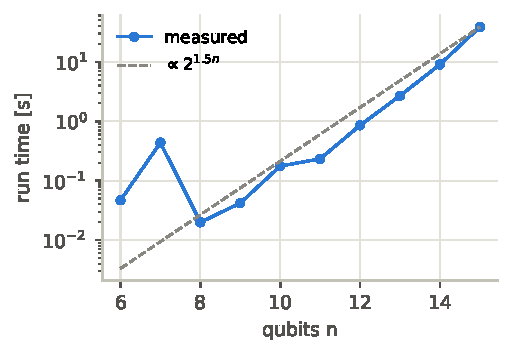
\includegraphics[width=0.78\textwidth]{benchmark_cpu}\\
      \raggedright\small
      One run per $n$ on the CPU (2000 shots). Theory: amplitudes double and iterations grow by $\sqrt2$ per qubit, so work $\propto 2^{1.5n}$. \hl{Timing depends on the machine}; small $n$ is dominated by overheads, and these are not general performance figures.
    \end{column}
  \end{columns}
\end{frame}

\begin{frame}{Resources as $n$ grows}
  \begin{columns}[c]
    \begin{column}{0.58\textwidth}
      \centering\small
      \begin{tabular}{rrrr}
        \toprule
        $n$ & $k_{\rm opt}$ & one state (fp64) & one state (fp32)\\
        \midrule
        15 & 142 & 512 KiB & 256 KiB\\
        20 & 804 & 16 MiB & 8 MiB\\
        25 & 4\,549 & 512 MiB & 256 MiB\\
        30 & 25\,735 & 16 GiB & 8 GiB\\
        33 & 72\,792 & 128 GiB & 64 GiB\\
        \bottomrule
      \end{tabular}\\[2mm]
      \raggedright\footnotesize Computed from $2^n \times 16$ or $8$ bytes and the exact rule for $k_{\rm opt}$. Not measured.
    \end{column}
    \begin{column}{0.39\textwidth}
      \begin{block}{Theoretical vs.\ practical}
        \small
        \key{Queries} grow like $2^{n/2}$.\\[1mm]
        \key{Simulation work} grows like $2^{1.5n}$: a classical simulator touches every amplitude for every gate.\\[1mm]
        So a simulated Grover run shows the algorithm is correct; it gives \hl{no speed-up over classical search}.
      \end{block}
    \end{column}
  \end{columns}
\end{frame}

\begin{frame}{Noise: why long circuits fail}
  \begin{columns}[c]
    \begin{column}{0.56\textwidth}
      \centering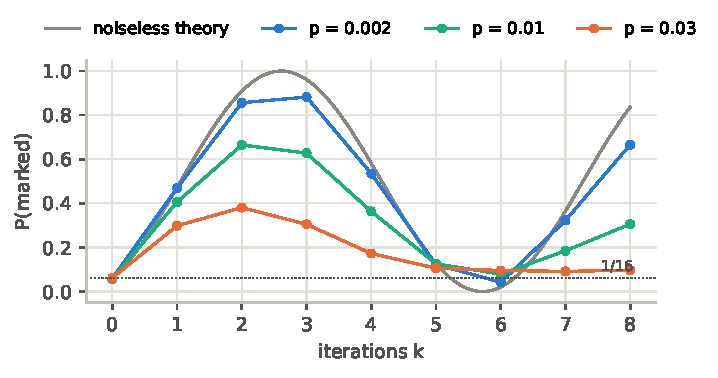
\includegraphics[width=\textwidth]{noise_n4}\\
      \small $n = 4$, CUDA-Q \texttt{density-matrix-cpu}, 4000 shots per point. Depolarising error $p$ after each $H$ and $X$ gate; multi-controlled gates are left noiseless. Illustrative only: not part of \texttt{Grover.ipynb}.
    \end{column}
    \begin{column}{0.4\textwidth}
      \begin{itemize}
        \item At $k = 3$: $P = \noisefour$, $\noiseone$, $\noisethree$ for $p = 0.002$, $0.01$, $0.03$ (noiseless: $0.961$).
        \item The signal decays and the state drifts to the uniform value $\frac1{16}$.
      \end{itemize}
      \begin{block}{Simple model}
        \small $P_k \approx f^k\sin^2((2k{+}1)\theta) + \frac{1 - f^k}{N}$. With $f = 0.99$ and $k = 25$: $P \approx 0.78$.
      \end{block}
    \end{column}
  \end{columns}
\end{frame}

\begin{frame}{Hardware considerations and limitations}
  \small
  \begin{itemize}
    \item \key{Depth}: $k \propto \sqrt N$ iterations, each with large multi-controlled gates. Current devices cannot run this for large $n$ without error correction.
    \item \key{Connectivity}: decomposing C$^{n-1}$Z on limited qubit connections adds many two-qubit gates.
    \item \key{The oracle}: the demonstration oracle already holds the answer. A useful oracle must compute $f$ reversibly, and can dominate the total cost.
    \item \key{Knowing $M$}: a wrong $M$ causes over-rotation; BBHT or counting are needed if it is unknown.
    \item \key{No sorted-data speed-up}: structured problems usually have better classical algorithms.
    \item \key{Data loading}: searching a stored database also needs a costly way to query it in superposition.
    \item \key{Simulation}: a state vector needs $2^n$ amplitudes, and the work grows like $2^{1.5n}$.
    \item \key{Parallelism}: $p$ machines save only a factor $\sqrt p$ in time (classically $p$).
  \end{itemize}
\end{frame}

\begin{frame}{Applications and future directions}
  \begin{columns}[T]
    \begin{column}{0.48\textwidth}
      \begin{block}{Cryptography}
        A $b$-bit key needs about $\frac\pi42^{b/2}$ iterations, and each runs the cipher reversibly. Doubling the key length restores the margin.
      \end{block}
      \begin{block}{Optimisation and constraints}
        Minimum finding (D{\"u}rr--H{\o}yer), SAT: a quadratic gain over brute force, not a polynomial algorithm.
      \end{block}
    \end{column}
    \begin{column}{0.48\textwidth}
      \begin{block}{Subroutine in other algorithms}
        Amplitude amplification, and amplitude estimation for Monte-Carlo-style sampling.
      \end{block}
      \centering\small
      \begin{tabular}{lc}
        \toprule
        task & queries\\
        \midrule
        search, classical & $\Theta(N)$\\
        search, quantum & $\Theta(N^{1/2})$\\
        2-to-1 collision & $\Theta(N^{1/3})$\\
        element distinctness & $\Theta(N^{2/3})$\\
        \bottomrule
      \end{tabular}\\[1mm]
      \raggedright\small \key{Directions}: resource estimates with error correction, cheaper oracles, fixed-point variants.
    \end{column}
  \end{columns}
\end{frame}

\begin{frame}{Where each result in these slides comes from}
  \centering\small
  \begin{tabular}{p{0.3\textwidth}p{0.62\textwidth}}
    \toprule
    kind & what\\
    \midrule
    \key{General theory} & Formulas and derivations. Several solutions, unknown $M$, exact and fixed-point search, amplification, counting, complexity bounds, decomposition with ancillas.\\[1mm]
    \key{Repository implementation} & One marked item; oracle from $X$ and \texttt{z.ctrl}; no ancillas; code listings from \texttt{build\_grover.py}.\\[1mm]
    \key{Illustrative examples} & Hand calculations with small $N$; the Toffoli oracle; the noise slide (same gates, with a noise model added for this lecture).\\[1mm]
    \key{Previously recorded} & 15-qubit run stored in \texttt{Grover.ipynb}: 2000/2000, 66.8\,s on 4 CPU cores.\\[1mm]
    \key{Newly executed} & CUDA-Q CPU runs by \texttt{make\_figures.py}: amplitudes, shots, 15-qubit re-run, benchmark, noise.\\[1mm]
    \key{Not validated} & GPU, multi-GPU, MPS, tensor-network and hardware options: present in the code, not run here.\\
    \bottomrule
  \end{tabular}
\end{frame}

\begin{frame}{Try it yourself: \texttt{Grover.ipynb}}
  \begin{columns}[T]
    \begin{column}{0.5\textwidth}
      \begin{enumerate}
        \item Install: \texttt{pip install -r requirements.txt}
        \item Open \texttt{Grover.ipynb} and run all cells.
        \item Change only Section 3:
          \begin{itemize}
            \item \texttt{N\_QUBITS} (default 15)
            \item \texttt{MARKED\_BITSTRING}: \texttt{"example"}, a bit string or an integer
            \item \texttt{GROVER\_ITERATIONS}: \texttt{"optimal"} or an integer
            \item \texttt{BACKEND}: \texttt{"cpu"}, \texttt{"gpu"}, \dots
          \end{itemize}
      \end{enumerate}
    \end{column}
    \begin{column}{0.46\textwidth}
      \begin{block}{Experiments}
        \begin{itemize}
          \item \texttt{N\_QUBITS = 4}: $k_{\rm opt} = 3$ and the whole circuit fits in the drawing
          \item \texttt{GROVER\_ITERATIONS = 284}: the marked item almost never appears ($P \approx 3\times10^{-6}$)
          \item \texttt{GPU\_PRECISION = "fp32"}: half the GPU memory
        \end{itemize}
      \end{block}
      The notebook compares results with $\sin^2((2k+1)\theta)$ and reports time and memory.
    \end{column}
  \end{columns}
\end{frame}

% =====================================================================================
\section{Part 8: Practice and summary}
\begin{frame}{Exercises}
  \begin{enumerate}
    \item Trace one iteration by hand for $N = 16$, one marked item. Give the marked amplitude and $P_1$.
    \item Find $\kopt$ and $P$ for $n = 5$, one marked item ($\theta = 0.1777$).
    \item Which $X$ gates does the oracle for $\ket{0110}$ need? How many gates has one iteration?
    \item $N = 64$ with $M = 16$. What is $P_1$? What about $M = 48$?
    \item The diffusion circuit gives $-D$. Why is the result still correct?
    \item With $k = 2\kopt$ on $2^{15}$ items, what do you expect to measure?
    \item How much memory does the notebook estimate for $n = 28$ with the sweep on: $4$, $8$ or $16$ GiB?
    \item Bonus: show that $D\Uo$ in the $\{\ket{r}, \ket{m}\}$ basis is a rotation by $2\theta$.
  \end{enumerate}
  \vspace{2mm}
  \small The Grover Question Paper has 80 further questions; the Answer Book explains every option.
\end{frame}

\begin{frame}{Answers}
  \small
  \begin{enumerate}
    \item Mean after the oracle $\frac{14}{16}\cdot\frac14 = \frac{7}{32}$. Marked: $\frac{7}{16} + \frac14 = \frac{11}{16}$. $\ P_1 = \frac{121}{256} \approx 0.473$.
    \item $\frac{\pi}{4\theta} - \frac12 = 3.92 \to 4$; $\ P = \sin^2 9\theta = 0.9992$.
    \item $X$ on qubits 1 and 4 (the zeros). $4n + 2z + 2 = 16 + 4 + 2 = 22$ gates.
    \item $M/N = \frac14$: $\theta = 30^\circ$, so $P_1 = 1$. $\ M/N = \frac34$: $\theta = 60^\circ$, so $P_1 = \sin^2 180^\circ = 0$.
    \item $-1$ multiplies the whole state: a global phase, which changes no probability.
    \item $569\,\theta = \pi + 0.0017$, so $P \approx 3\times10^{-6}$: almost never the marked item.
    \item One state $2^{28}\times16$ bytes $= 4$ GiB; the sweep doubles it: $8$ GiB.
    \item $\Uo = \mathrm{diag}(1, -1)$ and $D = \begin{psmallmatrix}\cos2\theta & \sin2\theta\\ \sin2\theta & -\cos2\theta\end{psmallmatrix}$. Multiplying gives $\begin{psmallmatrix}\cos2\theta & -\sin2\theta\\ \sin2\theta & \cos2\theta\end{psmallmatrix}$.
  \end{enumerate}
\end{frame}

\begin{frame}{Summary}
  \begin{columns}[T]
    \begin{column}{0.56\textwidth}
      \small
      \begin{itemize}
        \item \key{Unstructured search}: classically about $N/M$ queries; with Grover about $\frac\pi4\sqrt{N/M}$.
        \item \key{Oracle} $\Uo$ flips the sign of solutions. \key{Diffusion} $D = 2\pj{s} - I$ inverts about the mean.
        \item Two reflections make a \key{rotation by $2\theta$}, with $\sin\theta = \sqrt{M/N}$.
        \item $P_k = \sin^2((2k+1)\theta)$; $\ \kopt = \mathrm{round}(\frac{\pi}{4\theta} - \frac12)$; too many iterations \key{over-rotate}.
        \item Circuit: $H$ layer, then ($X$, C$^{n-1}$Z, $X$) and ($H$, $X$, C$^{n-1}$Z, $X$, $H$), repeated.
        \item The speed-up is quadratic and provably optimal.
      \end{itemize}
    \end{column}
    \begin{column}{0.4\textwidth}
      \begin{block}{Further reading}
        \small
        \begin{itemize}
          \item L.\,K.\ Grover, \emph{A fast quantum mechanical algorithm for database search} (1996)
          \item M.\,A.\ Nielsen, I.\,L.\ Chuang, \emph{Quantum Computation and Quantum Information}, Chapter 6
          \item Boyer, Brassard, H{\o}yer, Tapp, \emph{Tight bounds on quantum searching} (1998)
          \item NVIDIA CUDA-Q documentation
          \item This repository: \texttt{Grover.ipynb}, \texttt{book/}, \texttt{assessments/}
        \end{itemize}
      \end{block}
    \end{column}
  \end{columns}
\end{frame}

\end{document}
